\documentclass[conference]{IEEEtran}
\IEEEoverridecommandlockouts
% The preceding line is only needed to identify funding in the first
% footnote. If that is unneeded, please comment it out.

\usepackage{subcaption}
\usepackage{libertine}
\usepackage{lipsum}% http://ctan.org/pkg/lipsum
\usepackage{algorithm}% http://ctan.org/pkg/algorithm
\usepackage{algpseudocode}% http://ctan.org/pkg/algorithmicx
\usepackage{graphicx}
\usepackage[compatibility=false]{caption}% http://ctan.org/pkg/caption
\usepackage{booktabs}
\usepackage{cite}
\usepackage{url}
\usepackage{multirow}
\usepackage{pgfplots}
\usepackage{tikz}
\usetikzlibrary{matrix,fit,shapes,calc,positioning,shadows,arrows,shapes,backgrounds,decorations.markings,fadings}
\usepgfplotslibrary{statistics}
\usepackage{listings}
%\usepackage[caption=false, font=footnotesize]{subfig}
\renewcommand{\ttdefault}{pcr}
\lstset{
  basicstyle=\scriptsize\ttfamily,
  keywordstyle=\scriptsize\ttfamily\bfseries,
  language=C,             % choose the language of the code
  frame=single,              % adds a frame around the code
  aboveskip=0pt,
  belowskip=0pt,
  breaklines=true,           % sets automatic line breaking
  breakatwhitespace=true,   % sets if automatic breaks should only happen at
  showspaces=false,
  %numbersep=5pt,              % Abstand der Nummern zum Text
  %tabsize=2,                  % Groesse von Tabs
  %extendedchars=true,         %
  keywords=[2]{tcp, flag, threshold, track, count, seconds, classtype, sid}
}
\usepackage{balance}
\usepackage{wrapfig}
\usepackage{enumitem}
\usepackage{color, colortbl}
\definecolor{Gray}{gray}{0.9}
\usepackage[skins]{tcolorbox}

\newcommand{\tname}{\textsc{Syrius}} %% name of the technique
\newcommand{\ie}{i.e.}
\newcommand{\eg}{e.g.}
\newcommand{\aka}{a.k.a.}
\newcommand{\etal}{and colleagues}
\newcommand{\nids}{NIDS}
\newcommand{\metas}{Metasploit}
\newcommand{\suri}{Suricata}
\newcommand{\numrulessuri}{27.8K}
\newcommand{\percRulesWithContent}{93.5\%}
\newcommand{\numundetected}{\Fix{XX\%}}
\newcommand{\CodeIn}[1]{{\small{\texttt{#1}}}}
\newcommand{\MyComment}[1]{}

%% review
\newcommand{\Fix}[1]{{\textbf{[[}\color{magenta}#1}\textbf{]]}}
\newcommand{\Mar}[1]{{\textbf{[[Marcelo:~}\color{red}#1}\textbf{]]}}
\newcommand{\Luc}[1]{{\textbf{[[Lucas:~}\color{blue}#1}\textbf{]]}}
\newcommand{\Gui}[1]{{\textbf{[[Guilherme:~}\color{green}#1}\textbf{]]}}

\def\denseitems{
   \itemsep1pt plus1pt minus1pt
   \parsep0pt plus0pt
   \parskip0pt\topsep0pt}

%% numbers
\newcommand{\totoptions}{162}
\newcommand{\numproto}{11}
\newcommand{\totoptionsrelevant}{153}


%\usepackage{theorem}
\usepackage{amsmath,amssymb,amsfonts}
%\usepackage{algorithmic}
%% \usepackage{graphicx}
%% \usepackage{textcomp}
%% \usepackage{xcolor}

\def\BibTeX{{\rm B\kern-.05em{\sc i\kern-.025em b}\kern-.08em
    T\kern-.1667em\lower.7ex\hbox{E}\kern-.125emX}}
\begin{document}


%
% Add comments in the text
%
\newboolean{showcomments}
\setboolean{showcomments}{true}
%\setboolean{showcomments}{false}

\ifthenelse{\boolean{showcomments}}
  {\newcommand{\nb}[3]{
  {\color{#2}\small\fbox{\bfseries\sffamily\scriptsize#1}}
  {\color{#2}\sffamily\small$\triangleright~$\textit{\small #3}$~\triangleleft$}
  }
  }
  {\newcommand{\nb}[3]{}
  }

\title{Rule Synthesis for Rule-based Intrusion Detectors}

%% \title{Conference Paper Title*\\
%% {\footnotesize \textsuperscript{*}Note: Sub-titles are not captured in Xplore and
%% should not be used}
%% \thanks{Identify applicable funding agency here. If none, delete this.}
%% }

%% \author{\IEEEauthorblockN{1\textsuperscript{st} Given Name Surname}
%% \IEEEauthorblockA{\textit{dept. name of organization (of Aff.)} \\
%% \textit{name of organization (of Aff.)}\\
%% City, Country \\
%% email address or ORCID}
%% \and
%% \IEEEauthorblockN{2\textsuperscript{nd} Given Name Surname}
%% \IEEEauthorblockA{\textit{dept. name of organization (of Aff.)} \\
%% \textit{name of organization (of Aff.)}\\
%% City, Country \\
%% email address or ORCID}
%% \and
%% \IEEEauthorblockN{3\textsuperscript{rd} Given Name Surname}
%% \IEEEauthorblockA{\textit{dept. name of organization (of Aff.)} \\
%% \textit{name of organization (of Aff.)}\\
%% City, Country \\
%% email address or ORCID}
%% \and
%% \IEEEauthorblockN{4\textsuperscript{th} Given Name Surname}
%% \IEEEauthorblockA{\textit{dept. name of organization (of Aff.)} \\
%% \textit{name of organization (of Aff.)}\\
%% City, Country \\
%% email address or ORCID}
%% \and
%% \IEEEauthorblockN{5\textsuperscript{th} Given Name Surname}
%% \IEEEauthorblockA{\textit{dept. name of organization (of Aff.)} \\
%% \textit{name of organization (of Aff.)}\\
%% City, Country \\
%% email address or ORCID}
%% \and
%% \IEEEauthorblockN{6\textsuperscript{th} Given Name Surname}
%% \IEEEauthorblockA{\textit{dept. name of organization (of Aff.)} \\
%% \textit{name of organization (of Aff.)}\\
%% City, Country \\
%% email address or ORCID}
%% }

\pagestyle{plain}
\maketitle

\begin{abstract}
Network Intrusion Detection Systems (\nids{}) are popular tools to
defend against network attacks. These systems monitor the network
traffic and flag suspicious network behavior. Rule-based \nids\ do
that by checking the network traffic against a set of rules, which
become obsolete as attackers learn new strategies to circumvent
existing defenses. This paper proposes \tname{}, a novel approach to
synthesize rules for \textit{rule-based} \nids. \tname\ leverages
malicious (positive) and benign (negative) traffic 
%\rui{positive and negative traffic are first introduced here, withuot being explaiend.} 
and examples of trusted rules to create
rules for new attacks. \tname{} is organized as a pipeline of three components that
1)~create an over-specified seed rule, 2)~derive plausible rules from
the seed, and 3)~rank plausible rules. Experimental results provide
evidence that \tname\ is promising.
 \rui{the example is interesting, but this gives the 
feeling that the work is too preliminary} 
For example, it was
able to synthesize the correct rule in all cases we analyzed and
ranked the correct rule among the first five rules of the reported
ranking in \percTopFiveRanking\ of the cases.
\end{abstract}

%% \begin{IEEEkeywords}
%% component, formatting, style, styling, insert
%% \end{IEEEkeywords}

\section{Introduction}
\label{sec:intro}

Network Intrusion Detection Systems (\nids{}) are software systems
that monitor the network traffic for malicious behavior and act
accordingly by blocking messages or alerting humans about suspicious
events~\cite{Mitchell:2014:SID:2597757.2542049}. \nids{} are typically
placed behind a firewall, vetting the traffic that the firewall did
not block. Various open-source (\eg{}, Snort~\cite{snort} and
Suricata~\cite{suricata}) and commercial (\eg{},
SolarWinds~\cite{solarwinds} and IBM QRadar~\cite{qradar})
\nids\ implementations exist.

% given the amount of potential malicious traffic that exist on the Internet

This paper focuses on rule-based \nids{}, which are very popular in
industry~\cite{proofpoint-etpro,snort-rule-subscriptions}. A
\emph{rule-based intrusion detector}\MyComment{\footnote{\aka\ signature-based
  intrusion detector.}} checks if the network traffic matches a fixed
set of rules. Figure~\ref{fig:pingscan-example} shows an example rule
of Suricata~\cite{suricata}, a popular open-source \nids{}. A rule
describes a pattern in the traffic. The observation of that pattern in
the traffic indicates an attempt of a malicious individual
to attack a local network. This particular rule prescribes a method to
capture an Active Reconnaissance attack for discovering accessible
hosts in a network (see Section~\ref{sec:active-recon}).

Open-source \nids{}, like Snort~\cite{snort} and
Suricata~\cite{suricata}, provide rulesets for many existing
attacks. Unfortunately, attackers actively look for new mechanisms to
\begin{wrapfigure}[8]{r}{0.21\textwidth}
    \vspace{-2ex}  
    \centering
    \scalebox{0.9}{  
      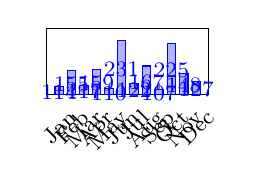
\begin{tikzpicture}
        \begin{axis}[
            width = 0.3\textwidth,
            height = 0.2\textwidth,            
            bar width=3pt,
            scaled ticks=false,
            ymajorticks=false,
            ybar stacked,
            ymax=250,
            enlargelimits=0.09,
            clip=true,
            legend style={at={(0.5,-0.15)},anchor=north,legend columns=-1},          
            xtick=data,
            xticklabel style={rotate=45, font=\footnotesize},
            tick pos=left,
            nodes near coords,
            every node near coord/.append style={font=\footnotesize},
            nodes near coords align={vertical},
            symbolic x coords={Jan, Feb, Mar, Apr, May, Jun, Jul, Aug, Sep, Oct, Nov, Dec},]
            \addplot coordinates {(Jan, 114) (Feb, 155) (Mar, 117) (Apr, 159) (May, 110) (Jun, 231) (Jul, 122) (Aug, 167) (Sep, 107) (Oct, 225) (Nov, 148) (Dec, 127)};
        \end{axis}
      \end{tikzpicture}
    }
    \vspace{-5ex}
    \caption{\label{fig:distribution-rules-per-month}2019 new rules.}
\end{wrapfigure}
exploit systems through the
network. Figure~\ref{fig:distribution-rules-per-month} shows the
number of rules added per month in the year of 2019 to the ``Emerging
Threats Open Ruleset''~\cite{emerging-threats-open}, a popular public
data set of \suri\ rules. A closer observation on the changelogs of
this ruleset~\cite{emerging-threats-changelogs} shows that new rules
are often created.  Rulesets need to be continuously revised as the
community finds and advertises vulnerabilities, which eventually can
be exploited by hackers.  Unfortunately, creating these rules is
time-consuming and error-prone~\cite{vollmer-etal-cics2011,alparslan-blog-suri}. The language for
describing rules is non-trivial (see
Section~\ref{sec:example-suricata-rules}) and testing correctness of a
rule requires data and careful inspection.

%% IT-security companies capitalize on this phenomena and
%% offer rulesets on the
%% market.

\sloppy This paper proposes \tname{} (for \textbf{Sy}nthesis of
Su\textbf{ri}cata R\textbf{u}le\textbf{s}), a technique to
automatically synthesize rules for rule-based \nids. Our goal is to
facilitate the creation of rules and, consequently, help system
administrators to harden the protection against network attacks.
\tname{} leverages different sources of information to synthesize
rules for a given attack. It uses 1) positive examples, \ie{},
scenarios that reproduce the attack, 2) negative examples in the form
of a data set of benign messages, and 3) a data set of human-written
trusted rules. The positive and negative examples constrain the search
space of rules that can be used to capture the attack. Intuitively,
positive examples indicate what should be captured whereas negative
examples indicate what should not be captured. It is worth noting that
classical machine learning techniques \emph{are not directly
  applicable in this context} as they typically have limited support
to string and structured data, which are prevalent in this domain.

%% vast amounts of negative data
%% exist~\cite{tcpreplay,stratosphere-normal}, but positive data is
%% scarce~\cite{} as it is not common (and considered unethical) to publish
%% attacks on the web\Mar{is there a term for non-deep web?}.

%Furthermore, \tname\ uses
%public data sets of rules to differentiate rules by the similarity to
%human-written rules.

\tname{} takes on input one or more examples \rui{We ought to explain how does one get hold on examples. How diffcult are they to obtain?} \Gui{Given a captured network traffic, an expert must identify which packets can be used to generate the rule. These packets are separated and given as input to Syrius.}of an attack and produces
on output a ranked list of rules for that attack. It uses public data
sets of benign messages~\cite{tcpreplay,stratosphere-normal} and
rulesets~\cite{emerging-threats-open} to create those rules. The
technique is organized as a pipeline of three components. First,
\tname\ uses the messages that manifest an attack to create a
potentially over-specified seed rule. Then, it uses that seed rule and
benign traffic to derive a set of plausible rules that isolate the
benign traffic from the malicious traffic. Finally, it uses existing
rules to learn heuristics to rank the plausible rules.

%\Mar{@Lucas, please look for constant
  %numbers as this *in text* and use macros instead. We do not want to
  %leave inconsistent data in the paper!}
We evaluated \tname\ against \totalAttacks attacks of various kinds, such as 
\Luc{This is already on section V, should it also be here?} Denial-of-Service (DoS)~\cite{denial-of-service},
Active Reconnaissance (AREC)~\cite{active-reconnaissance} and Privilege
escalation (PESC)~\cite{privilege-escalation}. %\Fix{...}\rui{add few examples}. 
The observed results are encouraging. For 
example, \tname\ ranked the correct rule among the top five rules in \Fix{fix values}
\percTopFiveRanking\ of the cases and ranked the correct rule among 
the top ten rules in \topTenAttacks of the \totalAttacks cases. \rui{to discuss, I find 
this a bit weak.}\Mar{agree. let us try to add more examples and data.}

%% \Fix{
%% denial-of-service
%% attack to a server by matching specific conditions about the network
%% traffic~\cite{understanding-dos}. Relevant properties about the
%% traffic of interest appear in bold in this rule (see
%% Section~\ref{sec:suri-metas-coverage}). Deployments of rule-based
%% \nids\ are restricted to a fixed set of rules defined by the network
%% system administrator.}



%% Note that anomaly-based \nids are evolving pretty quick with the
%% advances in machine learning, but rule-based \nids are still extremely
%% popular.  \tname{} could also leverage existing databases of malicious
%% traffic to synthesize rules.  Regardless of how the negative traffic
%% is produced (out of scope of this paper), those rules can be
%% distributed to rule databases for free.
%%  The
%% core motivation is that 1) attackers are productive in creating new
%% ways to circumvent existing protections and 2) manual creation of
%% rules is tedious and time-consuming.  

This paper makes the following contributions.

\newcommand{\Contrib}[1]{$\star$#1}
\begin{itemize}[topsep=.2ex,itemsep=.2ex,leftmargin=0.8em]

\item[\Contrib{}]\textbf{Approach.} A novel approach to synthesize
  rules for \nids.

\item[\Contrib{}]\textbf{Evaluation.} An evaluation of our approach on
  attacks of various kinds. Results indicate that \tname\ is effective
  in creating plausible rules and performs very well in ranking the
  correct rule among those generated.

\item[\Contrib{}]\textbf{Implementation.} A public implementation of
  \tname. (Available on request to preserve double-blindness.)

\item[\Contrib{}]\textbf{Data.} A data set of artifacts involved in
  the evaluation of \tname\ (\eg{}, pcap files of example attacks, list
  of plausible rules generated, etc.). The data set is available at
  the following URL~\ourdataset.
  
\end{itemize}


\section{\nids}
\label{sec:background}

This section presents background used in the next sections.

\subsection{Rule-based and Anomaly-based \nids}

\sloppy Network Intrusion Detection Systems (\nids{}) are typically
categorized in two groups~\cite{kumar2007survey}: rule-based, as
briefly described on Section~\ref{sec:intro}, and anomaly-based
\nids. An \emph{anomaly-based intrusion detector} learns usage
behavior from benign traffic and, based on that, alerts uncommon
traffic~\cite{7579764,kumar2007survey,Mitchell:2014:SID:2597757.2542049,cordy-etal-issta19}. Rule-based
\nids{} and anomaly-based \nids{} are complementary. A rule-based
\nids{} focuses on known attacks whereas an anomaly-based \nids{}
focuses on unknown potential attacks. Rule-based \nids\ can miss
attacks as rulesets can become obsolete whereas anomaly-based
\nids\ can report false alarms as learning algorithms that generalize
observations from benign traffic are approximate.  This paper focuses
on rule-based \nids\ for its popularity in industry. Although we used
Suricata, the principles we used are general to any other
signature-based \nids~(\eg{}, Snort~\cite{snort}).

%%  It
%% has been successfully used to identify denial-of-service
%% attacks. 
%% More
%% precisely, an anomaly-based \nids{} flags an attack when the traffic
%% on the network shows a different pattern compared with the historical
%% traffic.



%\vspace{-1ex}
\subsection{Suricata Rules}
\label{sec:example-suricata-rules}

%% \footnote{IPS (Intrusion Prevention System) and IDS differ in
%%   the action taken when an intrusion is observed. IPS systems block
%%   malicious traffic whereas IDS systems only alert them. However, IDS
%%   and IPS are similar in the approaches used to detect
%%   intrusions~\cite{ids-ips}.}

Figure~\ref{fig:pingscan-example} shows an example rule of
Suricata~\cite{suricata}, a popular open-source \nids{} maintained by
the Open Information Security Foundation (OISF)~\cite{oisf}.  A
Suricata rule is divided in three parts---action, header, and rule
options~\cite{suri-rule-format}. The \emph{action} appears as the
first word in the rule description---an \CodeIn{alert}, in this
case. An action denotes the task that needs to be executed if the
rule pattern is satisfied.  In this example, an alert message will be
sent to system administrators if the rule pattern is
satisfied. The \emph{header} comes after the
action in the rule description. It restricts the information flow
monitored by the rule. The header of this rule is \CodeIn{icmp any any
  -> any any}. It instructs Suricata to inspect \CodeIn{icmp} traffic
flowing from any machine and port to any machine and port.\MyComment{
  The variables \CodeIn{\$HOME\_NET} and \CodeIn{\$EXTERNAL\_NET} are
  configurable.} Finally, \emph{rule options} come after the
header. It is a semi-colon-separated sequence of key-value pairs. Rule
options serve to document the analyzed traffic (\eg{}, ``msg'',
``classtype'', and ``sid'') and to characterize the attack pattern
(\eg, ``flags'', ``threshold'', and ``content''). \tname{} produces
options of the second kind, which are \emph{relevant} to capture the
attack. For example, the option \CodeIn{content:<arg>} checks if the
argument is present in the payload of a message.

%\vspace{-1ex}
\begin{table}[t!]
  \footnotesize
  \caption{\label{table:rules}Example of capture-relevant options of Suricata.}
  \vspace{-2ex}
  \centering
  \begin{tabular}{clp{6cm}}
    \toprule
    \multicolumn{1}{c}{\#} & \multicolumn{1}{c}{Name} &  \multicolumn{1}{c}{Description}\\
    \midrule     
    1 & dsize & matches on the size of the packet payload\\
    2 & itype &  matches on a specific ICMP type\\
    3 & icode & matches on a specific ICMP code\\
    4 & icmp\_seq  & checks a ICMP sequence number\\
    5 & icmp\_id & matches on specific ICMP id-values\\
    6 & window & checks the size of the TCP window\\
    7 & flags & matches on TCP flags\\
    8 & fragbits & checks if the frag. bits are set in the IP header\\ % or reserved bits
    9 & threshold & min \# messages for a rule before it generates alerts\\
    10 & content & checks if argument is present on the payload\\
    \bottomrule
  \end{tabular}
  \vspace{-3ex}  
\end{table}

Table~\ref{table:rules} shows a sample of capture-relevant options of
Suricata. Column ``\#'' shows the option number, column ``Name'' shows
the name of the option, and column ``Description'' summarizes
purpose. The option \CodeIn{content} deserves special attention. It is
common in rules to capture http attacks and http rules are the most
common in the Emerging Threats Open
Ruleset~\cite{emerging-threats-open}. The content option takes a
sequence of bytes as argument and checks if that sequence appears in
the payload of the message.  For example, the option
\CodeIn{content:''SELECT''} checks if the string ``SELECT'' is present
in the payload.  Detailed description of the Suricata rules can be
found elsewhere~\cite{suri-rule-format}. Suricata supports a total of
\totoptions\ distinct options covering \numproto\ distinct network
protocols.


%% A total of 9 of these options
%% are for documentation.\MyComment{For instance, the purpose of rule
%%   option \CodeIn{msg} is to print on the output an informative message
%%   indicating what kind of intrusion has been observed.}
%% Figure~\ref{fig:distribution-rules-protocol} shows the distributions
%% of these options per protocol. The sum of the number of protocol
%% options is higher than \totoptions\ as some options are shared across
%% different protocols. \tname{} does not make distinction among protocols.


%% %\begin{wrapfigure}[14]{r}{0.5\textwidth}
%% \begin{figure}[t!]
%%   \centering
%% %  \vspace{-7ex}
%%   \scalebox{0.85}{
%%     \begin{tikzpicture}
%%       \begin{axis}[
%%           ybar stacked,
%%           enlargelimits=0.15,
%%           legend style={at={(0.5,-0.15)},
%%             anchor=north,legend columns=-1},
%%           %          ylabel={\#rules},
%%           symbolic x coords={dns, ftp, http, icmp, ip, smb, smtp, ssh,
%%           tcp, tls, udp},
%%           xtick=data,
%%           xticklabel style={rotate=45},          
%%           nodes near coords,
%%           every node near coord/.append style={font=\scriptsize},        
%%           nodes near coords align={vertical},
%%         ]
%%         \addplot coordinates {(dns,10) (ftp,11) (http,20) (icmp,18)(ip,16) (smb,13) (smtp,11) (ssh, 10) (tcp, 32) (tls,18) (udp, 18)};
%% %        \legend{relevant, irrelevant}
%%       \end{axis}
%%     \end{tikzpicture}
%%   }
%%   \vspace{-2ex}
%%   \caption{\label{fig:distribution-rules-protocol}Number of relevant
%%     options per protocol supported by Suricata.\Mar{not sure if this
%%       is really helpful.}}
%% %\end{wrapfigure}
%% \end{figure}
  

\subsection{Non-http Rules and Packets}
\label{sec:rules-and-packets}

%% We mentioned above that http rules often used content options, which
%% associate with the message payload.

Options of non-http rules typically associate with packet fields. Let
us consider a rule for an icmp attack as example.

\begin{figure}[h!]
  \centering
  \vspace{-2ex}  
  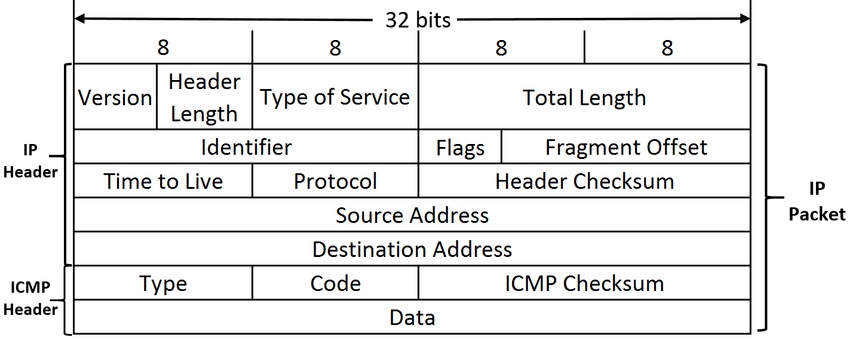
\includegraphics[scale=0.27]{figs/ICMP-packet-structure.png}
  \vspace{-1ex}
  \caption{Layout of an icmp packet.}
  \vspace{-1ex}
  \label{fig:icmp-packet-layout}
\end{figure}

Figure~\ref{fig:icmp-packet-layout} shows the
layout of an icmp packet. The packet fields ``Flags'' and ``Time to
Live'', declared in the ip header, are mapped to the \suri\ options
\CodeIn{fragbits} and \CodeIn{ttl}, respectively. Likewise, the fields
``Type'' and ``Code'', declared in the icmp header, are mapped to the
options \CodeIn{itype} and \CodeIn{icode}, respectively. The values of
the options ``ttl'', ``itype'', and ``icode'' are the same as the
value of the corresponding fields in the icmp packet. For the field
``Flags'' the value of the corresponding option is encoded in a
bitvector. For example, if the ``Flags'' field stores the value 101,
the corresponding rule option will be \CodeIn{fragbits:RM}, as each
position of the vector encodes a different character in the
\CodeIn{fragbits} option.

In summary, the value of several options \emph{of non-http rules} can
be determined through transformation functions, as those informally
described above. One exception to this is the option
\CodeIn{threshold}, which is typically used in denial-of-service
attacks. That option operates over sequence of messages as opposed to
single messages.

%Consequently, it is not possible to determine its
%values from a single message.


%% More precisely, to trigger an action on a rule
%% containing that option a \nids\ tool needs to monitor several
%% messages.

%% \Luc{
%%   Os campos Flags e Time to live no header IP são mapeados para as opções fragbits e ttl, respectivamente. Os campos Type e Code no header ICMP são mapeados para as opções itype e icode. \\
%% Os campos, Time to Live, Type e Code recebem diretamente o valor que está no pacote. Por exemplo, se o campo Type no pacote possuir valor 8, na regra ele vai aparecer como itype:8.\\
%% O campo Flags é intepretado como um vetor de bits, onde cada posição representa uma flag. Na regra, o valor do campo Flags é traduzido em caracteres que representam cada flag presente no pacote. Por exemplo: se o campo Flags possuir o valor 1010, na regra aparecerá fragbits:RM, pois os caracteres R e M indicam a presença do quarto e segundo bits.}


\section{Illustrative Example}
\label{sec:suri-metas-coverage}
\label{sec:active-recon}

This section briefly shows how \tname{} synthesizes rules for one
example attack. Active Reconnaissance is typically used as a
preliminary step towards an actual attack. It is a method to collect
information about a computing system to determine potential
vulnerabilities. For example, the Ping Scan attack~\cite{ping-scan}
scans the network for IPs of accessible hosts. An attacker sends
several ICMP Echo requests to a range of IP addresses in the network
and checks which ones respond to these requests. This method enables
an attacker to discover which machines are active in the network.

%\vspace{-1ex}
\begin{figure}[h!]
  \lstinputlisting[language=C,numbers=none,keywords={dsize,itype}]{pingscan.suricata}
  \vspace{-1ex}  
  \caption{Suricata rule for Ping Scan attack.}
  \vspace{-2ex}  
  \label{fig:pingscan-example}
\end{figure}

Figure~\ref{fig:pingscan-example} shows a Suricata rule that captures
Ping Scan, as documented on NMAP~\cite{netmap}, a network security
auditing tool. The essential options to capture the attack are in
bold---the option \CodeIn{dsize: 0} indicates that the packet has no
bytes in the payload and the option \CodeIn{itype: 8} indicates that
the packet to be captured are ICMP Echo requests.

%---in the form of network messages---
% one or more examples of an attack
%, indicating that the rule applies to \CodeIn{icmp}messages

In the following, we show how \tname{} synthesizes rules for this
attack. The main challenge in synthesizing rules is to discover the
set of rule options (see Table~\ref{table:rules}) that captures the
malicious traffic, but allows the benign traffic to pass. \tname{}
proceeds as follows to synthesize rule options.

%% \tname{} takes on input benign and malicious traffic and
%% produces on output rules to capture only the malicious
%% traffic. 

First, it analyzes the malicious traffic to extract rule's action,
header, and \emph{initial} options expressed in the
traffic. Considering the Ping Scan attack, \tname{} replays the
attack---with NMAP, in this case---and monitors the traffic.  It
infers the header by checking the protocol of the input messages. In
this case, \tname{} sets the header to \CodeIn{icmp any any -> any
  any}. It uses the most general flow description instructing the
\nids\ to analyze the icmp traffic flowing from/to any address and
port.  The rationale is that the choice of these parameters are
domain-specific and subject to change by the sys admins. Likewise,
\tname{} leaves the action of the corresponding rule constant, as
\CodeIn{alert}. Furthermore, recall from
Section~\ref{sec:rules-and-packets} that some options can be inferred
from packet contents. \tname{} finds the following five options at
this stage: {\scriptsize{\texttt{\textbf{dsize}:0; \textbf{itype:}8;
      \textbf{icode:}0; \textbf{icmp\_id:}23570;
      \textbf{icmp\_seq:}3439;}}}.  By construction, a rule that uses
this set of options captures the malicious traffic. Unfortunately, the
rule above is over-specified. Informally, the rule includes ``too
specific'' characteristics of the malicious traffic and could
potentially result in false negatives. In this case, although the
options \CodeIn{dsize:0} and \CodeIn{itype:8} are present in the set
of inferred options---as the golden rule from
Figure~\ref{fig:pingscan-example} shows---the others are not.


%% \vspace{-2.5ex}
%% \begin{figure}[h]
%%   \lstinputlisting[language=C,numbers=none,frame=none,keywords={dsize,icode,itype,icmp\_id,icmp\_seq}]{pingscan.suricata.synth}
%% \end{figure}
%% \vspace{-2.5ex}
%% \noindent


Second, \tname{} uses the benign traffic to mitigate the over-fitting
problem. In this step, \tname{} searches for alternative rules that
preserve the invariant to capture the positive (/malicious) traffic
but not capture the negative benign traffic. It uses the rule obtained
in the previous step as seed to bootstrap the search for alternative
plausible rules, \ie{}, rules that satisfy the aforementioned
invariant. The search is designed to generate rules containing subsets
of the options declared in the seed rule. Considering this example,
\tname{} produces a total of \pingscanplausible{} plausible rules at
the end of the search. This is a smaller number when compared to $2^n$
option combinations, where $n$ is the number of options contained in
the seed rule ($n=5$, in this case). \tname{} is able to prune the
search space and discard many implausible rules. It is worth noting
that the number of plausible rules that \tname\ produces at this step
can be very high for other example attacks. For illustration, see
column ``\#~Plausible Rules'' on Table~\ref{table:results}.


Finally, \tname{} ranks plausible rules according to heuristics
obtained by analyzing a database of existing rules. The general
intuition is that new rules should share characteristics with existing
human-written rules. For example, one heuristic function used by
\tname{} leverages the popularity of options for ranking. According to
that heuristic alone, the score of a rule $r$ is proportional to the
popularity of the options declared in
$r$. Figure~\ref{fig:distribution-options} shows the distribution of
options associated with rules from a public
ruleset~\cite{emerging-threats-open} containing
\numrulessuri\ rules. Note that rules with options \CodeIn{content}
and \CodeIn{flow} are the most common. The options \CodeIn{dsize} and
\CodeIn{itype}, the ones associated with the golden rule, appear as
the 6th and 7th most popular, respectively. Restricted to the set of
five options obtained at the first step, \CodeIn{dsize} and
\CodeIn{itype} are the most popular. At the end of this step, \tname{}
ranks the golden rule second in the list including
\pingscanplausible{} rules. It is worth noting that
\tname\ consistently ranks the golden rule very high in most of the
cases even when the technique produces a large number of plausible
rules (see Table~\ref{table:results}).

To sum up, \tname{} uses the messages that manifest an attack in the
first step to create a potentially over-specified seed rule. Then, it
uses benign traffic in the second step to create a set of plausible
rules from the seed rule. Finally, in the third step, \tname{} uses
existing rules to learn heuristics to rank plausible rules.

\section{Technique}
\label{sec:technique}

\tname{} is a technique to synthesize rules for rule-based
\nids~(\eg{}, Snort~\cite{snort} and Suricata~\cite{suricata}). The
goal is to automatically create rules that capture an attack of
interest.

\vspace{1ex}
\noindent\textbf{Overview.}~\tname\ takes on input one or more
examples of an attack and produces on output a ranked list of
\emph{plausible rules}, \ie{}, rules capturing only the malicious
traffic produced by the attacks. Figure~\ref{fig:overview} shows 
the workflow of \tname{} as a pipeline of three components, appearing 
numbered in the figure. As public data sets of benign
traffic~\cite{tcpreplay,stratosphere-normal} and rules
exist~\cite{emerging-threats-open}, a user of \tname{}
only needs to provide examples of attacks.

%% To create rules, \tname\ leverages (1)
%% benign and malicious network traffic and (2) rules from public
%% rulesets. 

\begin{figure}[t!]
  \centering
  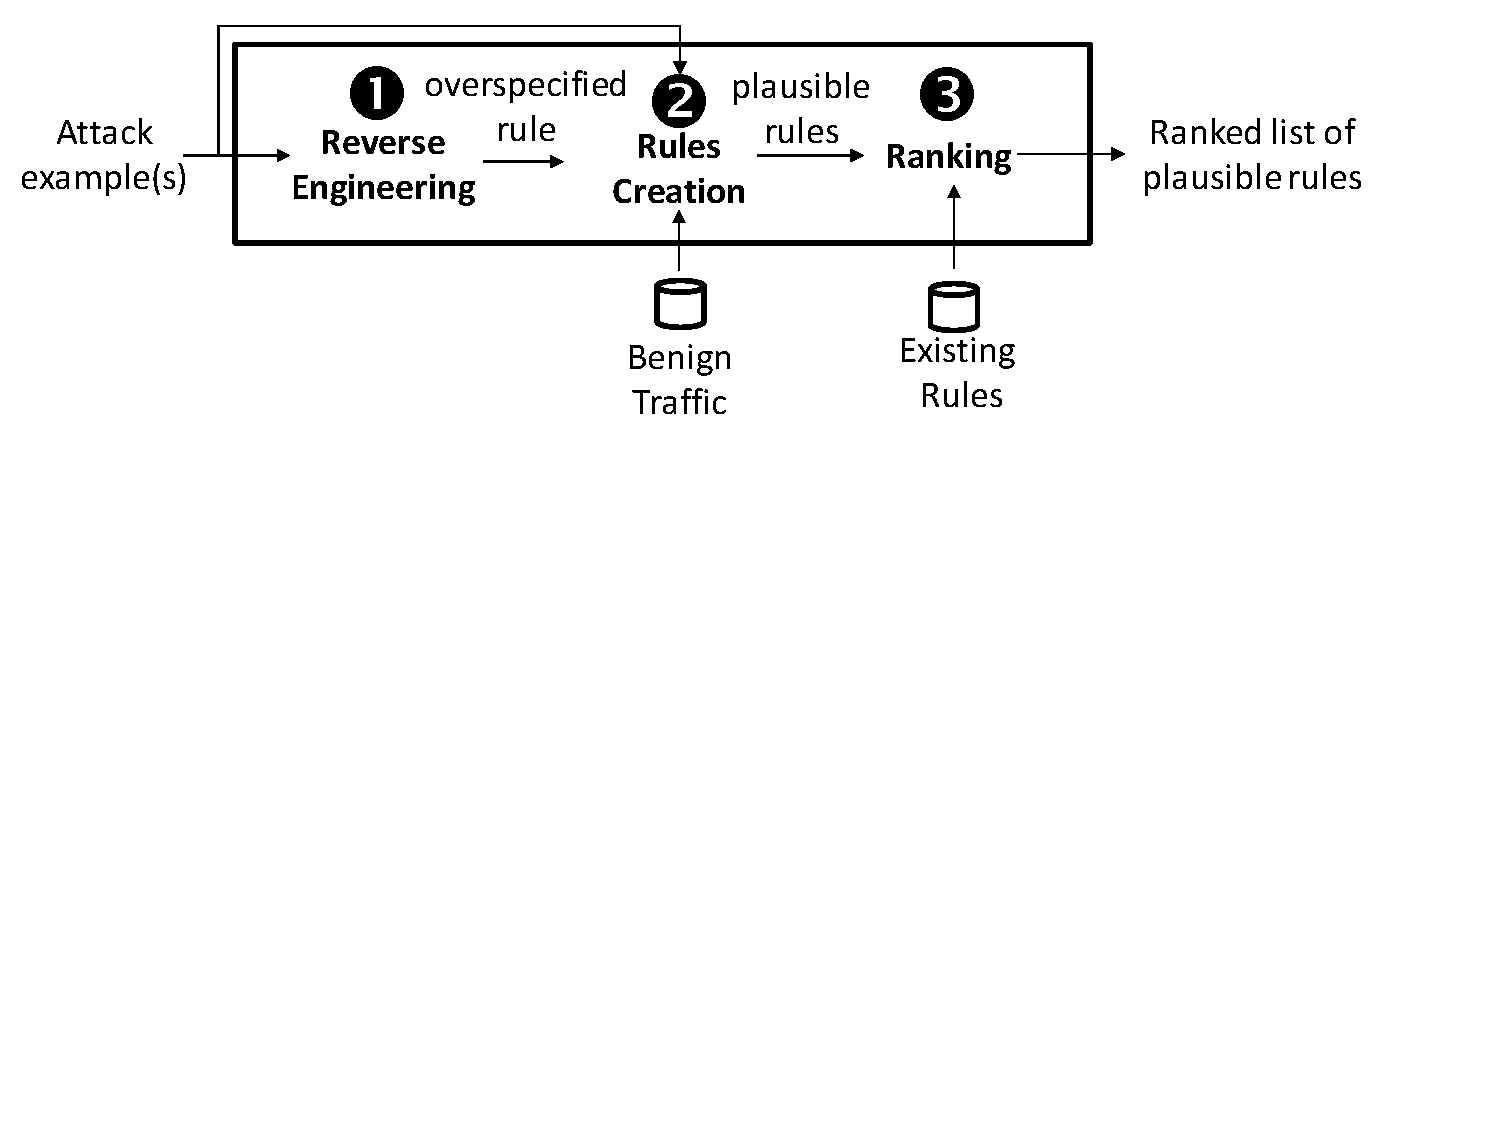
\includegraphics[trim=0 340 50 0,clip,width=0.48\textwidth]{figs/nids-workflow}
%  \vspace{-2ex}  
  \caption{The \tname\ workflow.}
  \label{fig:overview}
  \vspace{-4ex}
\end{figure}

% (see Section~\ref{sec:rules-and-packets})

%% However, note that that
%% approach alone could result in false positives as it imposes no limit
%% on the extent that the rules can be weakened.  More precisely, it
%% searches for plausible rules derived from the seed rule obtained in
%% the previous step. 

\tname\ works as follows. First, it creates a rule that captures the
malicious traffic associated with example attacks provided on
input. In this step, \tname\ detects options directly from the input
messages. More precisely, it creates a rule containing options that
are guaranteed to be satisfied by the malicious traffic. We refer to
that rule as the \emph{seed rule} and its corresponding set of options
as \emph{seed options}. It is important to note that, because only the
malicious traffic is considered in this step, the seed rule is
potentially over-specified, \ie{}, it may be more restrictive than
necessary. Consequently, the use of that rule could result in false
negatives. Second, \tname\ uses benign traffic to generate alternative
rules that 1) weaken the constraints expressed in the seed rule while
2) still capturing the malicious traffic. Given that every option
declared in a rule needs to be satisfied for a rule to capture an
attack, any subset of the set of seed options, by definition, captures
the attack characterized by the malicious traffic. \tname{} leverages
that observation to search for plausible rules containing a proper
subset of options from the seed options that captures \emph{only} the
malicious traffic. Finally, \tname{} uses heuristic functions,
obtained from a data set of existing rules, to rank the generated
plausible rules by their similarity to existing rules. Similarity is
used to approximate user's intent. The following sections detail each
component of \tname.

%%  As the generation
%% procedure discards options from the initial rule, the rules \tname{}
%% creates satisfy the property of capturing malicious traffic.



%% The goal of the first
%% component is to produce a rule that captures the negative traffic.
%% First, it initializes the rule with random values. Only options
%% associated with the used protocol are included in the rule
%% representation. Then, \tname\ optimizes the rule options until
%% \suri\ is able to capture the attack associated with the negative
%% traffic.  \tname\ unsuccessfully terminates at this point if it cannot
%% capture the attack. The second component takes as input the rule
%% produced by the first component and tries to minimize that rule. Note
%% that any subset of options would capture the negative traffic---as all
%% options in the rule need to be satisfied for the negative traffic to
%% be captured---but it can also capture positive traffic. This component
%% systematically discards options from the rule encoding until no
%% positive traffic is captured.



\subsection{Step 1: Reverse Engineering}
\label{sec:reverse-engineering}

The goal of the Reverse Engineering step is to infer a \emph{seed
  rule} that captures the attack. To that end, \tname{} monitors the
traffic produced by the input example attack(s) and extracts options
from related messages. A rule that contains these options captures the
malicious traffic by construction. \tname\ uses two strategies to
extract options: 1)~field and 2)~payload. The field strategy applies
to any protocol whereas the payload strategy applies only to http.
The decision of which strategy to use is based on the protocol
associated with input traffic--\tname{} uses the payload strategy if
http is detected; otherwise, it uses the field strategy. We elaborate
on these strategies in the following.

For the field strategy, \tname{} parses the input messages looking for
options associated with the data in the fields of
messages. Section~\ref{sec:rules-and-packets} shows the correspondence
between packet fields and some of the rule options from \suri\ and
Section~\ref{sec:active-recon} shows a concrete example where \tname{}
uses this strategy. Although we built the option-field mapping
manually, from the \suri\ documentation, this is a one-time activity.
Unfortunately, for http attacks, the relevant data for the options is
likely at the message payload; not the fields. By analyzing our data
set of rules, we found that this occurs frequently in http attacks,
which are prevalent. For example, \percHttp\ of the \numrulessuri{}
rules from the ruleset we analyzed~\cite{emerging-threats-open}
prescribe defenses against http attacks. In addition,
\percRulesWithContent{} of these rules contain at least one content
option. Figure~\ref{fig:rule-jboss} shows an example of a rule that
captures traffic containing the string \CodeIn{"/HtmlAdaptor"} in the
payload.  Figure~\ref{fig:distribution-contents} shows the
distribution of number of content options per rule for the data set
mentioned above. We limited the number of content options per rule to
10 in the histogram for space. \MyComment{Rules without
  \CodeIn{content} options are an exception and half of the rules
  contain at least two \CodeIn{content} options.}  To sum up, handling
content options for http is very important.

The content strategy focuses on extracting content options from the
message payload. By inspecting existing rules, we found that these
options refer to sequences of characters separated by natural language
delimiters such as $\backslash$t, $\backslash$n, $\backslash$r, and
spaces. To find the values associated with these options, \tname{}
splits the payload in tokens using these delimiters.

%Considering the example from Section~\ref{sec:active-recon},
%\tname{} produced a total of 5 tokens.

It is worth noting that we found that deciding which reverse
engineering strategy to use based on the protocol of the input
(malicious) messages showed to be effective. For
flooding attacks, \tname\ runs the same approach for each message and
identifies common options across all messages. For that case,
\tname\ reports, in addition, a \CodeIn{threshold} option, as
discussed on Section~\ref{sec:rules-and-packets}.  At the end of the
Reverse Engineering step, \tname\ produces a seed rule that captures
the malicious traffic.

%% \Mar{Nao esta muito claro como isto funciona. Rodamos sempre as duas
%%   estrategias (para obter field options e content options)?
%%   (Precisamos dizer se eh possivel ter regras com os dois tipos de
%%   opcoes). Como isto funciona 1) quando uma ataque tem varias
%%   mensagens (e.g., ping scan) e 2) quando temos varios ataques?}

%% \textbf{Implementation.}~
%% , characterized with pcap files~\cite{pcap}, a popular format
%% to describe network packets.

%% \Fix{
%% A avaliação que fazemos aqui pontua um dado content de acordo com
%% quantas vezes o campo em que ele se encontra eh referenciado nas
%% regras. Por exemplo, vamos supor que o tokenizer produziu a opção
%% content: "/HtmlAdaptor". Essa string pertence ao campo "Request
%% URI:". Esse campo pode ser acessado pelo modificador http\_uri. O
%% tokenizer associa o content a esse modificador.
%% }


\subsection{Step 2: Rules Creation}
\label{sec:minimization}

The seed rule produced in the first step satisfies the criterion to
capture the traffic produced by the example attacks. However, that
rule is over-constrained.  It may include options irrelevant to
capture the attack and lead to false negatives---the \nids\ may be
unable to capture manifestations of the same attack whose messages do
not exhibit the data satisfying irrelevant options. For example, the
seed rule produced after the Reverse Engineering step on the Ping Scan
example (Section~\ref{sec:active-recon}) contains options
\CodeIn{icode:0}, \CodeIn{icmp\_id:23570}, and
\CodeIn{icmp\_seq:3439}, which are irrelevant to capture that attack.

%%  Some options added to the rule
%% during the first step are irrelevant for determining the attack and
%% should be removed to obtain more general rules. 

To address the overfiting issue, \tname{} leverages public data sets
of benign traffic~\cite{tcpreplay} and additional examples of the
attack to guide the search for more general rules. To that end,
\tname{} \emph{minimizes} the rules produced in the previous step,
preserving the invariant of \emph{only} capturing the positive
malicious traffic. We say that a rule is minimal if discarding any
option results in the capture of negative (\ie{}, benign) traffic.
The procedure we propose in this step builds on the observation that
all options from the rule produced in the previous step are satisifed
by the traffic produced by the attack. Consequently, any subset of
these options also captures the attack. 

\algdef{SE}[DOWHILE]{Do}{doWhile}{\algorithmicdo}[1]{\algorithmicwhile\ #1}%
\algnewcommand\algorithmicforeach{\textbf{for each}}
\algdef{S}[FOR]{ForEach}[1]{\algorithmicforeach\ #1\ \algorithmicdo}
\algnewcommand\And{\textbf{and} }%
\setlength{\textfloatsep}{3pt}% Remove \textfloatsep
\begin{algorithm}[t!]
  %\noindent\hspace{-2ex}
  \flushleft{}\textbf{INPUT:} (over-constrained) seed rule $sr$, pcap
  files for benign traffic\\
  ($\mathit{bTr}$), pcap files for malicious traffic ($\mathit{mTr}$)\\
  %\noindent\hspace{-27.5ex} 
  \textbf{OUTPUT:} Set of minimized rules $\mathcal O$\\
%\vspace{-3ex}
\captionof{algorithm}{Rule creation algorithm}\label{algo1}
\begin{algorithmic}[1]
  \State $\mathcal R \gets \{\mathit{sr}\}$\Comment{initial population of candidate solutions.}\label{line-init}
  \State $\mathcal O \gets \emptyset$
  \Do\label{start-do-while}
      \State $\mathcal R' \gets \emptyset$ \Comment{new iteration. reset.}\label{init-rprime}
      \ForEach {$ro \in \mathcal R $}\Comment{analyze each candidate rule.}\label{start-foreach}
           \For {$i \gets 1$ to $N$}\Comment{mutate each rule $N$ times.}\label{start-for}
               \State $r \gets copy(ro)$\label{copy}
               \State $j\gets \mathit{rand}(0,\mathit{len}(r))$\label{choose-index}
               \State $r[j]\gets 0$\Comment{discard option $j$ in $r$}\label{delete-option}
               \If{$\mathit{isNew(r)} \And\mathit{isPlausible}(r, \mathit{bTr})$} 
                   \State $\mathcal R' \gets \mathcal R' \cup \{r\}$\label{line-progress}
               \EndIf
           \EndFor\label{end-for}
       \EndFor\label{end-foreach}
       \State $\mathcal R \gets \mathcal R'$\Comment{update new generation}\label{define-next-gen}
       \State $\mathcal O \gets \mathcal O \cup \mathcal  R$\Comment{remember all rules}\label{output-accum}
  \doWhile{$\mathcal R\not= \{\}$}\Comment{repeat until reaching a
    fixpoint}\label{end-do-while}\\
  \Return $\mathit{filter(\mathcal O, mTr)}$\label{filtering}
\end{algorithmic}
\end{algorithm}

The rule creation procedure \tname{} uses iteratively discards options
from rules, derived from the seed rule, using the negative traffic to
guide the search for minimal rules.  Algorithm~\ref{algo1} shows the
pseudocode for deriving these rules. The algorithm takes as input an
over-constrained rule $sr$, denoting the seed rule produced at the
Reverse Engineering step, and pcap files~\cite{pcap} to reconstruct
the benign traffic ($\mathit{bTr}$) and the malicious traffic
($\mathit{mTr}$). The algorithm produces on output a set of
alternative rules to $sr$ that captures every instance of the attack
(as per $\mathit{mTr}$), but does not capture any message from the
benign traffic (as per $\mathit{bTr}$).

Line~\ref{line-init} initializes the current population of individuals
(\ie{}, rules) $\mathcal{R}$ with the seed rule $sr$. We encode a rule
as a bitvector where each index in the vector represents one option;
the value assigned at a given position indicates whether or not the
option is present in the rule. One iteration of the outer loop
(lines~\ref{start-do-while}-\ref{end-do-while}) processes the current
population of individuals $\mathcal R$ and creates the next generation
$\mathcal R'$. Line~\ref{init-rprime} initializes the population of
individuals for the next generation. The inner loop
(lines~\ref{start-foreach}--\ref{end-foreach}) iterates through each
candidate rule in $\mathcal R$. The algorithm mutates each of these
rules $N$ times \rui{is N an input? How does one determine it in practice?}, discarding one rule option each
time. Line~\ref{copy} assigns a copy of the bitvector encoding
$\mathit{ro}$ to variable $r$. Function $\mathit{len}$ returns the
length of a vector and function $\mathit{rand(lo, hi)}$ randomly
chooses one integer value in the range $[lo, hi]$ defined by its
parameters. So, the expression $\mathit{rand(0, len(r))}$, appearing
at line~\ref{choose-index}, returns an index of the option in $r$ and
the statement at line~\ref{delete-option} deletes that option. The
call to $\mathit{isNew}$ checks if $r$ has not been previously
generated in another iteration whereas the call to
$\mathit{isPlausible}$ checks if the rule only captures positive
traffic, \ie{}, it checks that no message present in $\mathit{bTr}$ is
captured by $r$. If $r$ satisfies both criteria, it is added to
$\mathcal R'$, which denotes the next generation of individuals in the
search. After processing every candidate rule in $\mathcal R$, the
next generation of individuals is defined (line~\ref{define-next-gen})
and the set of discovered rules is updated (at
line~\ref{output-accum}).

The do-while loop terminates when no rule in the current generation of
individuals can be further reduced without violating the invariant
that a candidate solution should only capture positive traffic. This
means that execution of one iteration of the do-while loop has not
reached the statement declared at line~\ref{line-progress}, which adds
one element to the set $\mathcal{R'}$. As $\mathcal{R'}$ is
initialized empty, that set will remain empty at the end of the
execution of the loop from
lines~\ref{start-foreach}-\ref{end-foreach}. The algorithm returns the
rules from $\mathcal O$ that capture \emph{all} example attacks
provided on input (line~\ref{filtering}).

Note that the algorithm produces no rules in the last iteration. Rules
with a single option are produced in the second-to-last iteration. In
other iterations, rules with more than one option are produced. The
search induces a search tree with the seed rule $sr$ as root,
single-option rules as child nodes, and rules with more options as
internal nodes. The edges of the tree denote the ancestor relation
between a pair of rules. It is also worth noting that the algorithm
reports every rule in the tree instead of only those with one
option. The reason is that the traffic used to check plausibility is
limited by definition---reporting only minimal rules with respect to
that traffic could discard the correct rule.

In summary, the algorithm reports many rules that are plausible by
using the benign traffic to reduce the over-constrained rule produced
at the \reveng\ step. In the Raking step (Section~\ref{sec:ranking}),
\tname{} ranks the rules.

%Intuitively, rules dissimilar to (a very
%large set of) trusted rules rank low.

% this algorithm reports by their similarity to trusted rules

\textbf{Correctness argument.}~The algorithm reports rules that
capture only the positive traffic. Every rule created during the
search captures the attack associated with the input as every created
rule contains a proper subset of the options from the original rule
and all those options are, by definition, satisfied by the traffic
produced by the original attack. In addition, from the definition of
$\mathit{isPlausible}$, reported rules capture \emph{only} the
positive traffic. If negative traffic is captured, a rule is not added
to $\mathcal R'$. Consequently, it cannot be an element of $\mathcal
O$ and reported on the output. Finally, from the definition of
function $\mathit{filter}$, only the rules in $\mathcal O$ that
capture all the instances of the attack (\ie{}, variants) are reported
on output.



%% \begin{proposition}
%%   The minimization algorithm may not produce minimal rules.
%% \end{proposition}

%% \begin{proof}
%% The output of the minimization algorithm may contain rules that are
%% not minimal given the non-determinism of the algorithm. In principle,
%% it is possible that options that could be discarded are not selected
%% in the loop from lines~\ref{start-for}--\ref{end-for}. However, we
%% found empirically that a small value of $N$ suffices to discard those
%% options from a rule.
%% \end{proof}

%% Public databases of negative traffic with
%% \Fix{thousands} of messages exist  and can be used to
%% increase the accuracy of the minimization.
%\subsection{Limitations}
%\Fix{...}

\textbf{Implementation details.} We implemented function
\emph{isPlausible} by 1)~spawning Suricata to monitor a specified
rule, 2)~replaying the benign traffic (see
Section~\ref{sec:dataset-benign}), and 3)~reading the Suricata logs to
check if any benign message was captured by the rule. The function
\emph{filter} is implemented similarly. It returns a projection of the
set $\mathcal O$ where every rule captures the attacks characterized
by $\mathit{mTr}$. It is worth noting that Suricata can process
\emph{pcap} files~\cite{pcap} very efficiently compared to analyzing
network messages directly. Instead of sending traffic to a machine
with a deployed server (\eg{}, web server) that \suri\ would monitor,
our setup calls \suri\ directly through an API. \suri\ is invoked
multiple times for creating rules.

%% \textbf{Limitations.} It is worth
%% noting that the performance of \tname{} depends on the quality of
%% inputs. For the positive malicious traffic, \tname{} only requires one
%% sample (as input to step one), but can benefit of several samples (see
%% line~\ref{filtering} of Algorithm~\ref{algo1}). The same applies to
%% the negative traffic. However, in this case, \tname{} can use a large
%% variety of public data sets available online (see
%% Section~\ref{sec:objectanalysis-benign}).

\rui{paragraph on complexity? I wonder whether that is a good ideia because
this is already a long section.}

\subsection{Step 3: Ranking}
\label{sec:ranking}

\tname{} uses a composition of heuristic functions to rank the rules
produced in the previous step. Each of these functions uses a
different criterion to estimate how similar a new rule is to the rules
from public rulesets (\eg{},~\cite{emerging-threats-open}). The
intuition is that rules that look more similar to existing trusted
rules are more likely to reflect user's intention and be more
useful. The aggregated score of a rule is the weighted average across
the values produced by each heuristic function. The co-domain of each
function ranges on the 0-1 interval. Hence, the score of a rule also
ranges on the 0-1 interval. We describe in the following each of these
heuristic functions.

%% \Luc{atualmente eh uma
%%   média simples e não ponderada ja q as funções tem o mesmo
%%   peso. conversamos na ultima reuniao sobre testar diferentes pesos
%%   para cada função, mas n sei quão prioritário eh isso comparado as
%%   outras atividades que definimos.} $\sum{f_i}/|f_i|$.

%% Note that there are 11 rules with no
%% options. These rules only use the header to signal a traffic as
%% malicious. Also note that most rules have 2 to 6 options. 

\subsubsection{\label{sec:popularity-options}Popularity of options}

\tname{} use the popularity of the options used in trusted rules as a
heuristic function---rules containing popular options score higher
compared to those containing unpopular
rules. Figure~\ref{fig:distribution-options} shows the histogram of
rule options for the ruleset we used~\cite{emerging-threats-open}. The
x-axis shows the options used in rules (the 10 most common) and the
y-axis shows the number of rules using the corresponding option. Note
that the options \CodeIn{content}, \CodeIn{flow}, and \CodeIn{prce}
are very popular. \tname\ uses the following formula to compute the
contribution of option popularity to the score of a rule $r$:
\indent
$\sum_{i=1}^{N}\frac{\mathit{option\_frequency[option_i]}}{\mathit{max(option\_frequency)}}/N$.

%% {\small
%% \vspace{-2ex}
%% \[


%% \]
%% \vspace{-2ex}
%% }

\noindent
The term $\mathit{option_i}$ denotes the $i$th option in the bitvector
encoding $r$. The term $\mathit{option\_frequency}$ encodes the
distribution of option popularity as a dictionary mapping numbers,
indicating popularity, to corresponding options. The expression
$\mathit{option\_frequency[option_i]}$ denotes the number of rules,
from our dataset, containing $\mathit{option\_i}$. The expression
$\mathit{max(option\_frequency)}$ refers to the maximum number of
rules for any dictionary entry (to normalize the measurement in the
0-1 range), and $N$ is the number of options in $r$. To illustrate,
the contribution of this function to the score of a rule would be
$0.26=$($10181$+$3049)/(2$*$25699)$ for a rule with options
\CodeIn{prce} and \CodeIn{flowbits} and
$0.01$=$(155$+$108)/(2$*$25699)$ for a rule with options
\CodeIn{itype} and \CodeIn{icode}.

%% \Gui{A quinta heuristica que utilizamos
%%   considera a popularidade das opcoes. Primeiro pegamos a quantidade
%%   de vezes que uma opcao eh utilizada (sem considerar repeticoes numa
%%   unica regra). Dividimos o valor encontrado para cada opcao pelo
%%   maior valor encontrado, encontrando sempre valores de no maximo
%%   1. Entao na regra nos somamos os valores de cada opcao, dividido
%%   pelo numero de opcoes, chegando a um numero de no maximo 1, que
%%   representa a popularidade das opcoes na regra.}

%% \subsubsection{Size of a rule}
%% \label{sec:heuristic-size-of-rule}
%% \tname{} values rules in that size range higher compared to
%% other sizes.

%% We calculate the contribution of size of a given rule
%% $r$ with the  $\mathit{rules\_per\_size}[\mathit{len(r)}]/\mathit{max(rules\_per\_size)}$, where $\mathit{len(r)}$ denotes the number of options of a rule $r$,
%% $\mathit{rules\_per\_size}$ encodes the distribution of sizes as a
%% dictionary mapping sizes to number of associated rules, and
%% $\mathit{max(rules\_per\_size)}$ returns the maximum number of rules
%% for any dictionary entry as to normalize the measurement in the 0-1
%% range. 
%% Consequently, the contribution of size is proportional to its
%% popularity. The contribution of this heuristic would be 0.684
%% (=3,662/5,353) to a rule with three options and 0.028 (=154/5,353) to
%% a rule with nine options.




%% \vspace{-2ex}
%% \[\]
%% \vspace{-2ex}
%\noindent

%% \Luc{Se for preciso temos numeros para fundamentar isso
%%   melhor, sao cerca de 70K contents nas 28K regras do
%%   data set}\Mar{sim, isto ajuda, porem mais importante eh saber quantas
%%   (\%) das 28K regras tem contents.} \Luc{92\%}

\pgfplotsset{width=6cm,compat=1.8}
\pgfplotsset{every tick label/.append style={font=\tiny}}

%%   \begin{subfigure}{.25\textwidth}
%%     \centering
%%     \scalebox{0.8}{
%%       \begin{tikzpicture}
%%         \begin{axis}[
%%           bar width=4pt,
%%           scaled ticks=true,
%%           ymajorticks=false,
%%           ybar stacked,
%%           enlargelimits=0.08,
%% %          enlargelimits=false,
%% %          axis equal,
%%           clip=false,
%%           legend style={at={(0.5,-0.15)},anchor=north,legend columns=-1},          
%%           xtick=data,
%% %          xticklabel style={rotate=45},          
%%           nodes near coords,
%%           every node near coord/.append style={font=\scriptsize},
%%           xticklabel style={font=\footnotesize},          
%%           nodes near coords align={vertical},
%%           symbolic x coords={0, 1, 2, 3, 4, 5, 6, 7, 8, 9, 10},
%%           ]
%%           \addplot coordinates {(0,11) (1,1301) (2,4910) (3,3662) (4,3250) (5,5353) (6,2911) (7, 1337) (8, 1246) (9,763) (10, 495)};
%%         \end{axis}
%%       \end{tikzpicture}
%%     }
%%     \vspace{-1ex}
%%     \caption{\label{fig:distribution-rule-size}Rule sizes.}
%%   \end{subfigure}%

\begin{figure*}[t!]
  \centering
\begin{subfigure}{.25\textwidth}
  \centering
  \scalebox{0.8}{  
    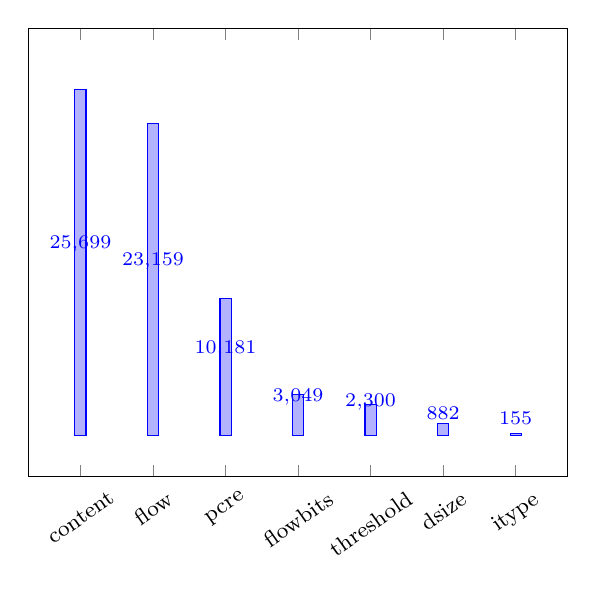
\begin{tikzpicture}
      \begin{axis}[
          bar width=4pt,
          scaled ticks=true,
          ymajorticks=false,
          ybar stacked,
          ymax=27000,
          enlargelimits=0.12,
%          enlargelimits=false,
%          axis equal,
          clip=false,
          legend style={at={(0.5,-0.15)},anchor=north,legend columns=-1},          
          xtick=data,
          xticklabel style={rotate=35},
          nodes near coords,
          every node near coord/.append style={font=\scriptsize},
          xticklabel style={font=\footnotesize},          
          nodes near coords align={vertical},
          %symbolic x coords={content, flow, pcre, flowbits, threshold, dsize, itype, icode, flags, tls.fingerprint},          
          symbolic x coords={content, flow, pcre, flowbits, threshold, dsize, itype},          
        ]
        \addplot coordinates {(content,25699) (flow,23159) (pcre,10181) (flowbits,3049) (threshold,2300) (dsize,882) (itype,155)};
      \end{axis}
    \end{tikzpicture}
  }
  \vspace{-5ex}
  \hspace{4ex}
  \caption{\label{fig:distribution-options}Option popularity.}
%  \vspace{-1ex}    
\end{subfigure}%  
  \begin{subfigure}{.25\textwidth}
    \centering
    \scalebox{0.85}{  
      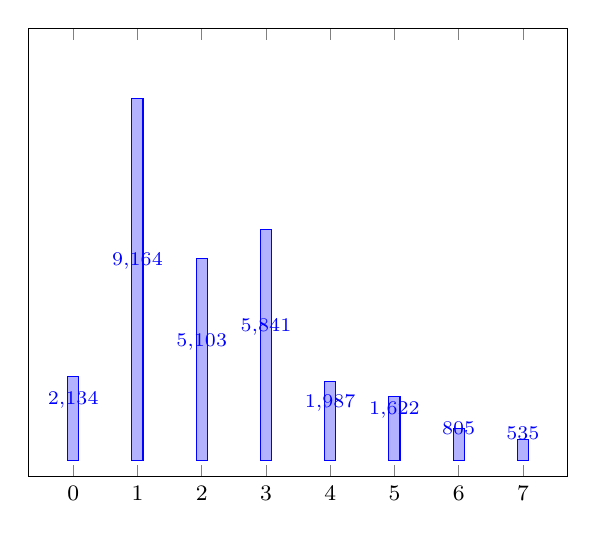
\begin{tikzpicture}
        \begin{axis}[
          bar width=4pt,
          scaled ticks=true,
          ymajorticks=false,
          ybar stacked,
          ymax=10000,
          enlargelimits=0.1,
%          enlargelimits=false,
%          axis equal,
          clip=false,
          legend style={at={(0.5,-0.15)},anchor=north,legend columns=-1},          
          xtick=data,
%          xticklabel style={rotate=45},          
          nodes near coords,
          every node near coord/.append style={font=\scriptsize},
          xticklabel style={font=\footnotesize},          
          nodes near coords align={vertical},
          %symbolic x coords={0, 1, 2, 3, 4, 5, 6, 7, 8, 9, 10},
          symbolic x coords={0, 1, 2, 3, 4, 5, 6, 7},
          ]
          \addplot coordinates {(0,2134) (1,9164) (2,5103) (3,5841) (4,1987) (5,1622) (6,805) (7, 535)};
        \end{axis}
      \end{tikzpicture}
    }
    \vspace{-1ex}
    \caption{\label{fig:distribution-contents}Number of content options.}
  \end{subfigure}% <---- don't forget this %
%  \\
\begin{subfigure}{.25\textwidth}
  \centering
  \scalebox{0.8}{  
    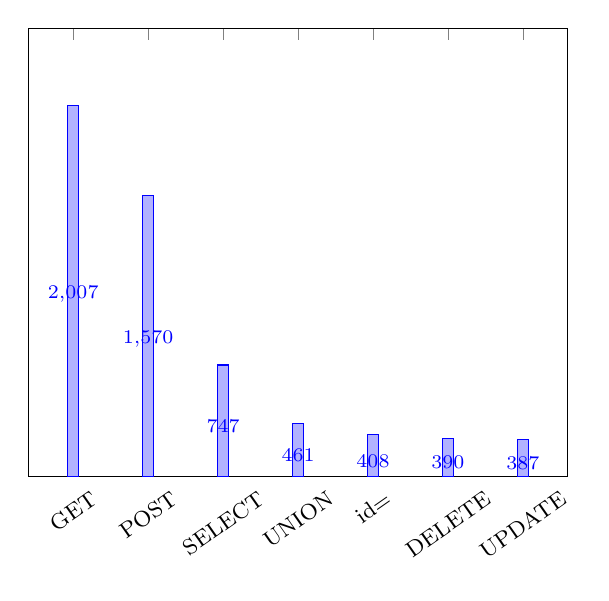
\begin{tikzpicture}
      \begin{axis}[
          bar width=4pt,
          scaled ticks=true,
          ymajorticks=false,
          ybar stacked,
          ymax=2200,
          enlargelimits=0.1,
%          enlargelimits=false,
%          axis equal,
          clip=false,
          legend style={at={(0.5,-0.15)},anchor=north,legend columns=-1},          
          xtick=data,
          xticklabel style={rotate=35},          
          nodes near coords,
          every node near coord/.append style={font=\scriptsize},
          xticklabel style={font=\footnotesize},          
          nodes near coords align={vertical},
          %symbolic x coords={GET, POST, SELECT, UNION, id=, DELETE, UPDATE, INSERT, 200, /index.php?},          
          symbolic x coords={GET, POST, SELECT, UNION, id=, DELETE, UPDATE},          
        ]
        \addplot coordinates {(GET,2007) (POST,1570) (SELECT,747) (UNION,461) (id=,408) (DELETE,390) (UPDATE,387)};
      \end{axis}
    \end{tikzpicture}
  }
  \vspace{-2ex}  
  \caption{\label{fig:distribution-strings}Strings used in content options.}
\end{subfigure}%
\begin{subfigure}{.25\textwidth}
  \centering
  \scalebox{0.8}{
    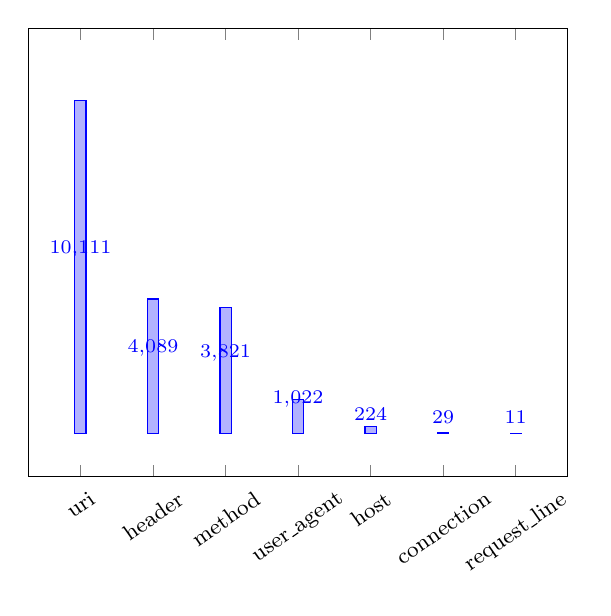
\begin{tikzpicture}
      \begin{axis}[
          bar width=4pt,
          scaled ticks=true,
          ymajorticks=false,
          ybar stacked,
          ymax=11000,
          enlargelimits=0.12,
%          enlargelimits=false,
%          axis equal,
          clip=false,
          legend style={at={(0.5,-0.15)},anchor=north,legend columns=-1},          
          xtick=data,
          xticklabel style={rotate=35},          
          nodes near coords,
          every node near coord/.append style={font=\scriptsize},
          xticklabel style={font=\footnotesize},          
          nodes near coords align={vertical},
          symbolic x coords={uri, header, method, user\_agent, host, connection, request\_line},          
        ]
        \addplot coordinates {(uri,10111) (method,3821) (user\_agent,1022) (header,4089) (host,224) (connection,29) (request\_line,11)};
      \end{axis}
    \end{tikzpicture}
  }
  \vspace{-2ex}
  \caption{\label{fig:distribution-content_modifiers}Http content modifiers.}
\end{subfigure}%
\vspace{-1ex}
\caption{Distributions.}
\vspace{-4ex}
\end{figure*}


\subsubsection{Number of content options} We observed
that \percContentOptions\ of the rules from the ruleset we analyzed
contain content options, but the distribution of those contents per
rule is not uniform. Figure~\ref{fig:distribution-contents} shows the
distribution of number of contents in a rule. Results indicate that
nearly 73\% of the rules from our ruleset contain one to three content
options. Hence, we found that that information could help
\tname\ discriminate useful rules. \tname{} computes the contribution
of the number of content options to the score of a rule $r$ with the
fraction
$\frac{\mathit{rules\_per\_number\_of\_contents[len(r)]}}{\mathit{max(rules\_per\_number\_of\_contents)}}$,
where $\mathit{len(r)}$ denotes the number of content options in $r$
and $\mathit{rules\_per\_number\_of\_contents}$ is the distribution of
number of contents. The expression in the numerator
%$\mathit{rules\_per\_number\_of\_contents[len(r)]}$
calculates the number of rules in the ruleset with the same number of
contents as $r$ whereas the denominator normalizes the value in the
0-1 range. To illustrate, the contribution of this function would be
$.64$~($=5841/9164$) and $.18$~($=1622/9164$) to the score of rules
with 3 and 5 options, respectively.

%% \noindent
%% The only difference of this formula compared to the one defined on
%% Section~\ref{sec:heuristic-size-of-rule} is the distribution used. The
%% distribution is given by the term
%% $\mathit{rules\_per\_number\_of\_contents}$ denoting a dictionary of
%% number of content options to number of rules that contain that number
%% of content options.

%% {\small
%% \vspace{-1.5ex}
%% \[
%% \]
%% \vspace{-0.5ex}
%% }

\subsubsection{Popularity of content strings} 
This heuristic leverages content rarity to discriminate rules. It
weighs higher (respectively, lower) rules that use popular
(respectively, unpopular) strings in content options. The score of a
rule $r$ on this function is the arithmetic mean of the popularity
scores of each string used in contents in $r$. More precisely, content
rarity is obtained with the following formula:
\indent
$\sum_{i=1}^{N}\frac{\mathit{content\_frequency[content_i]}}{\mathit{max(content\_frequency)}}/N$

\noindent
where $\mathit{content_i}$ denotes the $i$th content in a given
rule, the term $\mathit{content\_frequency[\mathit{content_i}]}$
denotes the frequency of the string used in the $i$th content, the
term $\mathit{max(content\_frequency)}$ denotes the maximum frequency
observed across all strings appearing as content parameters, and $N$
is the number of content options in a given
rule. Figure~\ref{fig:distribution-strings} shows the distribution of
the ten most popular strings in our ruleset. To illustrate, consider a
rule whose content options use the strings ``GET'' and ``ID''. The
contribution of that rule for the computation of similarity score
would be $0.601$ $(=(1$+$.203)$/$2)$. The relatively high weight
reflects the fact that ``GET'' and ``ID'' are popular content strings.

\begin{wrapfigure}[9]{r}{0.21\textwidth}
  \vspace{-2ex}
\centering
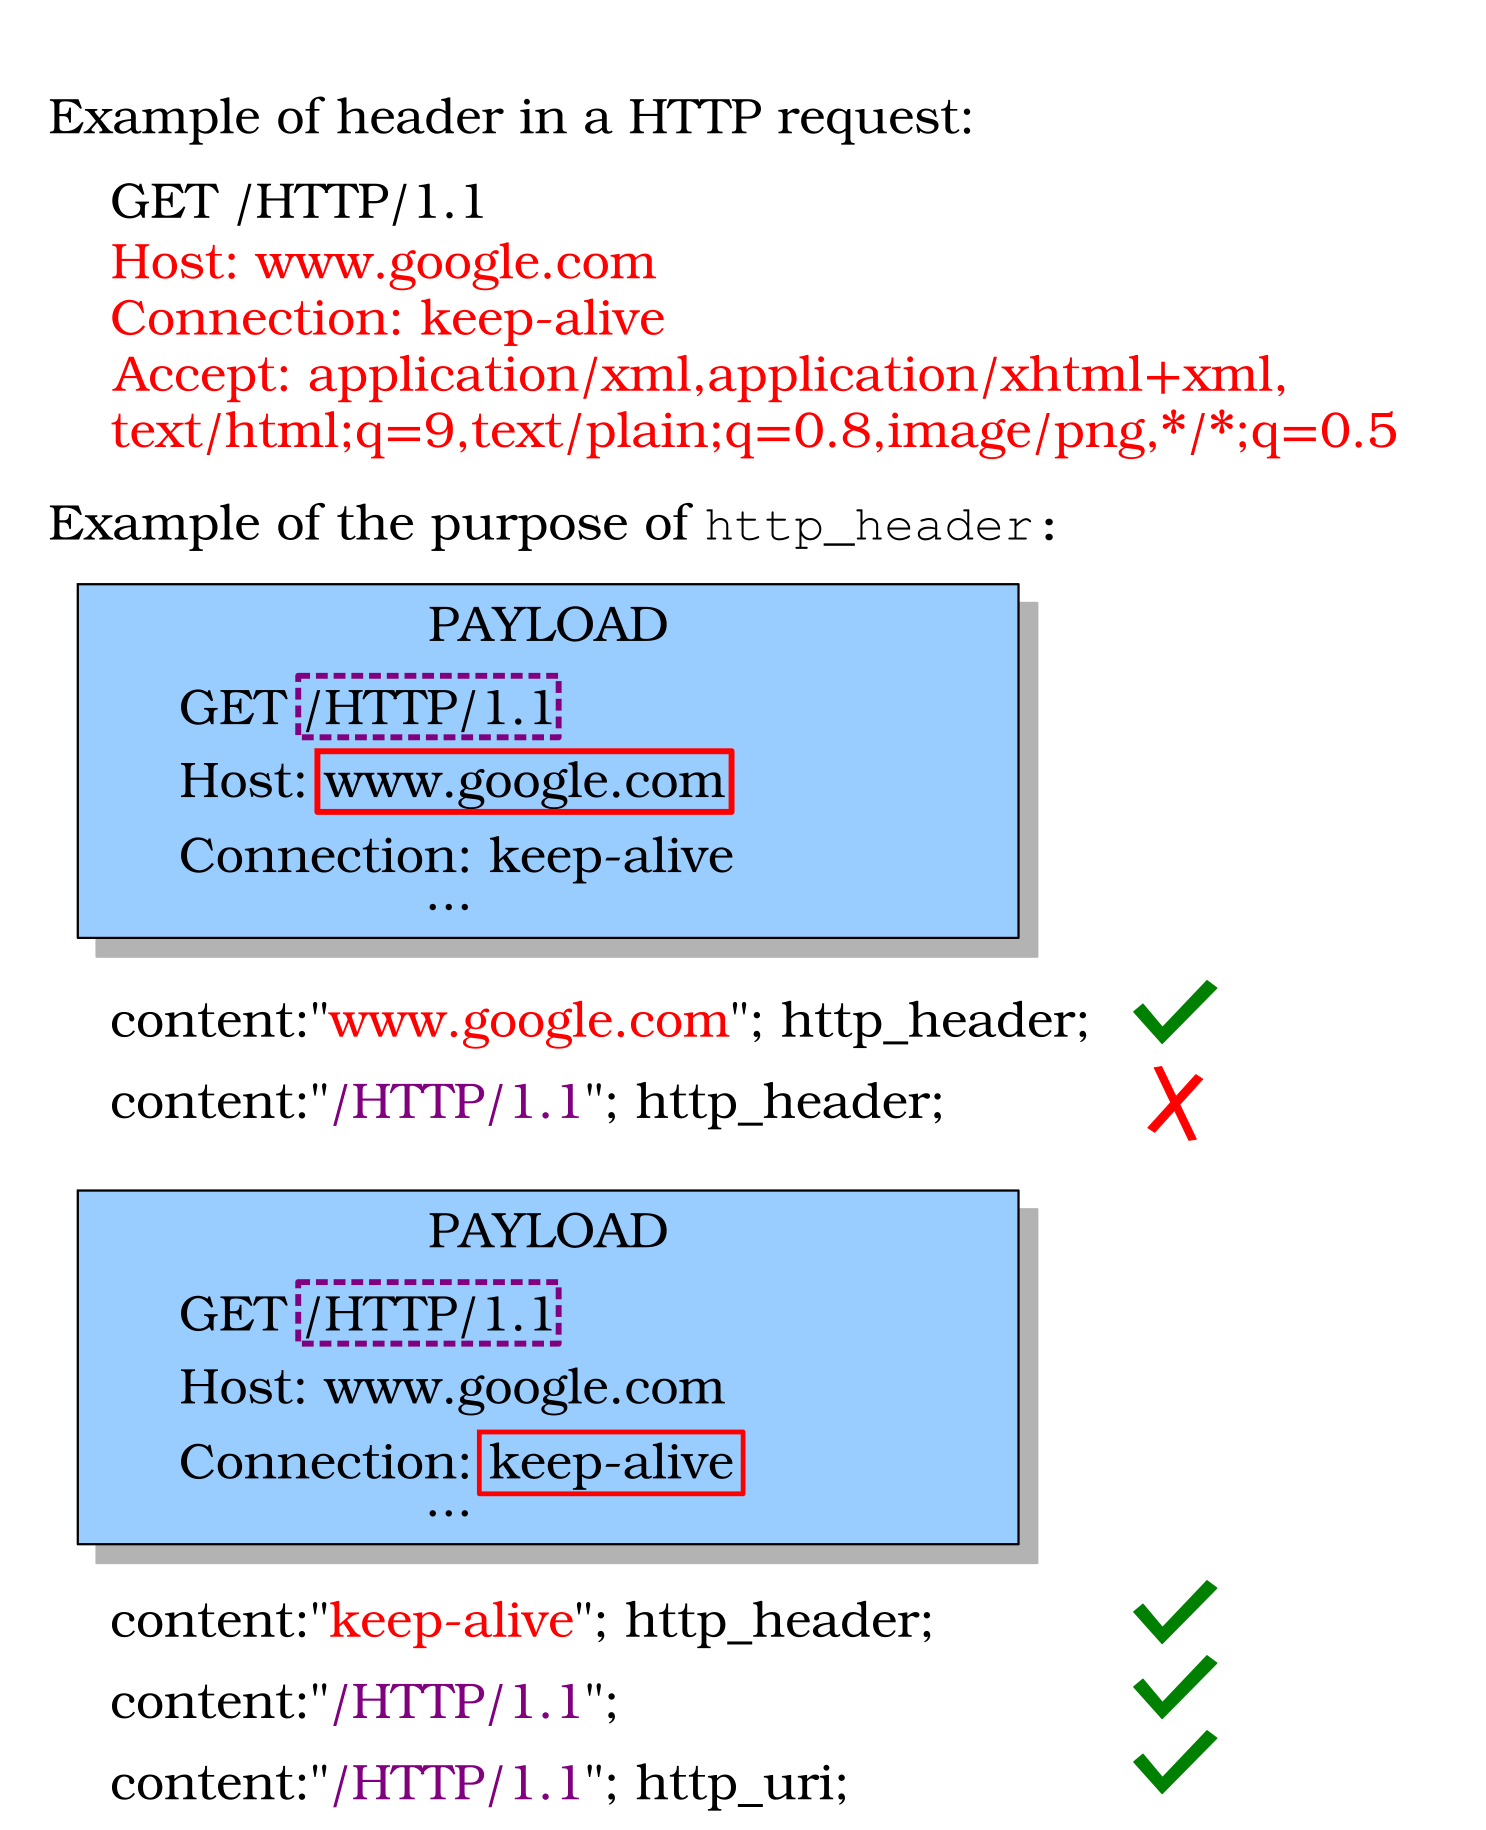
\includegraphics[scale=0.6]{figs/http_header-example.png}
\vspace{-1ex}
\caption{Content modifiers.}
\label{fig:http-header-example}
\end{wrapfigure}

\subsubsection{\label{sec:popularity-content-modifiers}Popularity of http content modifiers} As previously
mentioned, \percRulesWithContent\ of \suri\ rules involve content
options. Furthermore, nearly half of the rules that use content
options use content modifiers to qualify the search. Http modifiers
typically serve to specify parts of the message payloads that the
input string should be matched against. For example, the modifier
\CodeIn{http\_header} in the option \CodeIn{content: ``keep-alive'';
  http\_header} indicates that the string ``keep-alive'' should be
present in the header of the http message. (A keep-alive connection
attribute indicates that a single tcp connection should remain open
for multiple http requests/responses.) In this case, the content
modifier refers to an http field that appears in the payload of a tcp
message, which is the target of the option
\CodeIn{content}. Figure~\ref{fig:http-header-example} illustrates
possible content options used to match against certain strings that
appear in an http message. A check mark (respectively, cross)
indicates a match (respectively, no match).
\tname\ builds on the observation that the strings commonly accessed
at positions associated with content modifiers (\eg{}, host,
connection) are more common. For example, historical data indicates
that content options that use the modifier \CodeIn{connection} are
much less likely than content options that use the modifier
\CodeIn{uri}. Figure~\ref{fig:distribution-content_modifiers} shows
the histogram of content modifiers for http. (We removed the prefix
\CodeIn{http} on the modifier for space.) Although content modifiers
are applicable to rules of any protocol supported by Suricata,
currently, \tname\ only supports this features for tcp and http; these
rules comprise $\sim$80\% of the rules of our data set. We compute the
heuristic function for content modifiers with the following formula:

\indent
$\sum_{i=1}^{N}g(i)/N,~g(i)$=$\sum_{j=1}^{M_i}\frac{\mathit{modifier\_frequency[modifier_{ij}}]}{\mathit{max(modifier\_frequency)}}/M_i$


\noindent
where $g(i)$ is the contribution of content option $i$ to the score,
$N$ is the number of contents options present in a rule,
$\mathit{modifier\_frequency[modifier_{ij}}]$ denotes the popularity
of a modifier $j$ to content option $i$,
$\mathit{max(modifier\_frequency)}$ refers to the modifier with
maximum popularity (for normalization), and $M_i$ is the number of
content modifiers that could access the string associated with content
$i$.
To illustrate, consider a rule containing the option
\CodeIn{content:``/HtmlAdaptor''} (see Section~\ref{sec:jboss}). The
contribution of this option (\ie{}, the value of $\mathit{g(i)}$) to
the score of the rule is $0.5$ (=$\frac{10,111+11}{10,111*2}$). The
value of $M_i$, in this case, is 2 as the string ``/HtmlAdaptor''
could be accessed through the modifiers \CodeIn{uri} and
\CodeIn{request\_line}. The reason is that \tname\ identifies that
that string appears in the field \CodeIn{Request URI} (of an http
message from the malicious traffic) and that field is accessible
through these two modifiers. The relatively high heuristic value
reflects the fact that the string could be accessed by two popular
content modifiers.

%%%%%%%%%%%%%%
%% Removed for space
%%%%%%%%%%%%%%


%% As another example, consider the option
%% \CodeIn{content: ``keep-alive''}. In this case, either the modifier
%% \CodeIn{header} or the modifier \CodeIn{connection} could be used to
%% locate the string ``keep-alive'', stored in the field
%% \CodeIn{Connection} from an http message (see
%% Figure~\ref{fig:http-header-example}). Consequently the contribution
%% of this heuristic function to the corresponding rule would be $0.2$
%% (=$\frac{4089+29}{10111*2}$), in this case. Assuming that a rule uses
%% the two content options mentioned above, the aggregated contribution
%% of this heuristic function to the rule would be 0.35 (=(0.2+0.5)/2).

\subsubsection{Weight Optimization}
\label{sec:weight-optimization}
We optimized the weights of these heuristic functions as follows. We
ran \tname{} using different combinations of weights on a sample of
attacks and chose the combination that offered the best overall
performance, which we computed with the sum of the rankings of the
golden rule on each attack. The weight combination that led to the
smaller sum of rankings was considered the best choice. We considered
\emph{all} combinations of the following weights 0, 0.25, 0.5, 0.75,
and 1. Given that there are four different functions and five possible
weight values, we needed to run \tname{} on the sample of attacks for
625 (=$5^4$) times. In the end of the process, the weight combination
$\langle{}1,0.25,0.25,1\rangle$ was the best choice we found. Although
results showed that this strategy results in good performance, we
remain to evaluate other optimization strategies to find better
weights.

%% , such as evolutionary alternatives as
%% AVM~\cite{10.1109/32.57624}.
 
%\Gui{Fizemos um teste para encontrar melhores pesos para cada ataque. Calculamos o fitness de cada regra atribuindo diferentes pesos para cada função heurística. Os valores atribuídos foram 0, 0.25, 0.5, 0.75 e 1. Depois de calculado, ordenamos todas as listas criadas e pegamos a posição da Golden Rule. As melhores combinações de pesos (que conseguiram melhor posição da golden rule) estão na tabela 4, onde na coluna "Weights", há quatro números separados por vírgula, cada um deles representando o peso de uma função (na ordem que é representado no paper. O total de regras criadas é igual ao da Tabela 3.}


%\setlength{\tabcolsep}{5pt}
%renewcommand{\arraystretch}{0.9}
\begin{table*}[t!]
  \footnotesize
  \caption{\label{table:attacks}List of attacks. Non-http attacks
    appear at the top; http attacks appear at the bottom.}
  \vspace{-2ex}
  \centering
  \setlength{\tabcolsep}{4.5pt}
  \renewcommand{\arraystretch}{0.35}
  \begin{tabular}{lcccp{11cm}}
    \toprule
    \multicolumn{1}{c}{Name} &
    \multicolumn{1}{c}{Source} &
    \multicolumn{1}{c}{Type} &
    \multicolumn{1}{c}{Protocol} &
    \multicolumn{1}{c}{Groud Truth (relevant/checked options)} \\
    \midrule
    Black Nurse & \cite{pcap-attacks} & DoS & icmp & \textbf{icode}:3; \textbf{itype}:3; \textbf{threshold}: type both, track by\_dst, count 250, seconds 1;\\    
    Ping Scan & \cite{netmap} & AREC & icmp & \textbf{dsize}:0; \textbf{itype}:8; \\
    SYN Flood & \cite{hping3} & DoS & tcp & \textbf{flags}: S,12;
    \textbf{threshold}: type both, track by\_dst, count 5000, seconds 5;\\
    UDP Teardrop & \cite{udp-teardrop-source} & DoS & udp & \textbf{fragbits}:M; \textbf{id}:124; \\
      2100384 & \cite{iscx} & ICMP Info & icmp & \textbf{icode}:0; \textbf{itype}:8; \\
      2100399 & \cite{iscx} & ICMP Info & icmp & \textbf{icode}:1; \textbf{itype}:3; \\
      2100401 & \cite{iscx} & ICMP Info & icmp & \textbf{icode}:0; \textbf{itype}:3; \\
      2100402 & \cite{iscx} & ICMP Info & icmp & \textbf{icode}:3; \textbf{itype}:3; \\
      2100408 & \cite{iscx} & ICMP Info & icmp & \textbf{icode}:0; \textbf{itype}:0; \\
      2100485 & \cite{iscx} & ICMP Info & icmp & \textbf{icode}:13; \textbf{itype}:3; \\
      2100486 & \cite{iscx} & ICMP Info & icmp & \textbf{icode}:10; \textbf{itype}:3; \\
    %%UDP Flood & MazeBolt & DoS & UDP & \textbf{fragbits}:M; \textbf{threshold}: type both, track by\_dst, count 5000, seconds 5; \\
    \midrule
    %%Apache Struts 2 & \cite{wrccdc} & RCE & http & \textbf{content}:"POST"; http\_method; \textbf{content}:"java.lang.ProcessBuilder"; nocase; http\_client\_body; fast\_pattern; \textbf{content}:"/struts2-rest-showcase/orders/3"; http\_uri; \\    
    ColdFusion \MyComment{PESC} & \cite{nikto} & PESC & http \MyComment{& Privilege Escalation} & \textbf{content}:"GET"; http\_method; nocase; \textbf{content}:"/CFIDE/administrator"; http\_uri; nocase; \\
    iisadmin access\MyComment{web-application-attack} & \cite{nikto} & RCE & http \MyComment{& Adicionar} & \textbf{content}:"/iisadmin"; nocase; http\_uri; \\
    JBoss JMX\MyComment{ Console Beanshell Exploit} & \cite{nikto} & RCE & http \MyComment{& Remote Code Execution} & \textbf{content}:"/HtmlAdaptor"; nocase; http\_uri; \textbf{content}:"action=inspect"; nocase; http\_uri; \textbf{content}:"bean"; nocase; http\_uri; \textbf{content}:"name="; http\_uri; \\
    scripttag\MyComment{Possible Cross Site Scripting Attempt} & \cite{nikto} & RCE & http \MyComment{& Adicionar} & \textbf{content}:"</script>"; nocase; http\_uri; \\
    WeBid LFI \MyComment{Local File Inclusion} & \cite{nikto} & LFI & http & \textbf{content}:"GET "; depth:4; \textbf{content}:"/cron.php?"; http\_uri; nocase; \textbf{content}:"include\_path="; http\_uri; nocase; \textbf{content}:"../"; \\
    %%WordPress Login & \cite{wrccdc} & PVE & http & \textbf{content}:"log="; http\_client\_body; \textbf{content}:"\&pwd="; http\_client\_body; \textbf{content}:"\&wp-submit="; http\_client\_body; \\
    .htaccess access\MyComment{attempted-recon} & \cite{nikto} & AREC & http \MyComment{& Adicionar} & \textbf{content}:".htaccess"; nocase; http\_uri; \\
    .idq access\MyComment{EXPLOIT ISAPI} & \cite{nikto} & RCE & http \MyComment{& Adicionar} & \textbf{content}:".idq"; nocase; http\_uri; \\
    /system32/ in URI\MyComment{Possible Protected Directory Access Attempt} & \cite{nikto} & AREC & http \MyComment{& Adicionar} & \textbf{content}:"/system32/"; nocase; http\_uri; \\
    Basebuilder LFI & \cite{nikto} & LFI & http & \textbf{content}:"GET"; http\_method; \textbf{content}:"/main.inc.php?"; nocase; http\_uri; \textbf{content}:"mj\_config[src\_path]="; nocase; http\_uri; \\
    Tomcat Snoop Access & \cite{nikto} & AREC & http & \textbf{content}:"/jsp/snp/"; http\_uri; \textbf{content}:".snp"; http\_uri;\\  
    \bottomrule
  \end{tabular}
  \vspace{-2ex}
\end{table*}


\section{Evaluation}

This section reports on the evaluation of \tname{}.


\newcommand{\textRQone}{How well \tname\ ranks the golden rule?}
%\vspace{0.2cm}
\begin{itemize}[leftmargin=*,label={}]
\item{\textbf{RQ1.}} \textRQone
\end{itemize}

\noindent
\textbf{Rationale.}~The golden rule is a trusted human-written
\nids\ rule that we obtained from credible sources~\cite{emerging-threats-open}. 
\tname\ generates several rules that satisfy the invariant to only capture the malicious
traffic, but the amount of data we used to evaluate that property,
albeit large, is limited. Assessing the quality of each rule
\tname\ produces (\ie{}, fitness to the attack) requires domain
knowledge and much effort. The position of the golden rule at the
ranking produced by \tname\ is a proxy measure to the effort of a
system administrator in finding the rule that fits the purpose.


\newcommand{\textRQtwo}{How important are the heuristic functions
  to \tname's performance?}
%\vspace{0.2cm}
\begin{itemize}[leftmargin=*,label={}]
\item{\textbf{RQ2.}} \textRQtwo\
\end{itemize}

\noindent
\textbf{Rationale.}~We proposed a variety of heuristic functions to
rank the plausible rules that \tname\ created during minimization (as
per step 2 in the workflow). Recall that these functions are based on
the data from a public ruleset~\cite{emerging-threats-open} (see
Section~\ref{sec:ranking}). It is therefore important to understand
the extent to which each function contributes to the overall
performance of the technique.

\newcommand{\textRQthree}{How sensitive \tname\ is to the amount of
  positive examples?} \rui{should we also investigate the impact of the negative ones?}
%\vspace{0.2cm}
\begin{itemize}[leftmargin=*,label={}]
\item{\textbf{RQ3.}} \textRQthree\
\end{itemize}

\noindent
\textbf{Rationale.}~\tname\ uses both positive and negative examples
to generate rules. This question investigates how sensible the
technique is to the selection of these inputs.
\noindent
\vspace{1ex}

The following sections describe the objects we used to evaluate the
technique (Section~\ref{sec:dataset-benign}), answer the posed
research questions (sections~\ref{sec:answer-rqone},
and~\ref{sec:answer-rqtwo}, and~\ref{sec:answer-rqthree}), and
discuss threats to the validity of the
experiments~(Section~\ref{sec:threats}).


%%\begin{table}[h!]
%%  \small
%%  \caption{\label{table:weight}Weight Combinations.}
%%  \centering
%%  \begin{tabular}{lrrp{15cm}}
%%    \toprule
%%    \multicolumn{1}{c}{Name} &
%%    \multicolumn{1}{c}{Weights} &
%%    \multicolumn{1}{c}{Rank} \\
%%    \midrule
%%    Ping Scan & - & - \\
%%    SYN Flood & - & - \\
%%    JBoss JMX & 1,0,1,1 & 107 \\
%%    WetedhhtedBid & - & - \\    
%%    ColdFusion & 0,1,1,1 & 7 \\
%%    .htaccess access & 0,1,1,1 & 11 \\
%%    .idq access & 0,1,1,1 & 7 \\
%%    iisadmin access & 0,1,1,1 & 2 \\
%%    /system32/ in URI & 0,1,1,1 & 11 \\
%%    scripttag & 0,1,1,1 & 9 \\
%%    \bottomrule
%%  \end{tabular}
%%\end{table}
%%

\newcommand{\numNonContentAttacks}{4}
\newcommand{\numContentAttacks}{10}

\subsection{Objects of Analysis}
\label{sec:dataset-benign}
\label{attack-reproduction}
\label{subsec:malicious-traffic}
\label{sec:objectanalysis-benign}

%This section describes the objects used in the evaluation.

%\vspace{0.5ex}
\noindent\textbf{Attacks.}~Table~\ref{table:attacks} shows the selection
of attacks we analyzed.  Non-http attacks are listed at the top of the
table and http attacks are listed at the bottom. Recall from
Section~\ref{sec:reverse-engineering} that (1) http attacks are
prevalent, (2) most http attacks use only content options, and (3)
most non-http attacks only use field options. We selected
\numNonContentAttacks\ non-http attacks and \numContentAttacks\ http
attacks. The higher number of http attacks reflects their
popularity. Column ``Name'' shows the name of the attack, column
``Source'' shows the source where we obtained data to reproduce the
attack (see Section~\ref{subsec:malicious-traffic}), column ``Type''
shows the kind of attack, column ``Protocol'' shows the name of the
protocol explored in the attack, and column ``Ground Truth'' shows the
rule options to capture the attack. The rationale for the selection
were (1) to cover various kinds of attacks and (2) to cover attacks of
various protocols. Considering (1), the selection includes attacks of
the following types: Denial-of-Service (DoS)~\cite{denial-of-service},
Active Reconnaissance (AREC)~\cite{active-reconnaissance}, Privilege
escalation (PESC)~\cite{privilege-escalation}, Remote Code Execution
(RCE)~\cite{remote-code-execution}, Local File Inclusion
(LFI)~\cite{local-file-inclusion} and ICMP Traffic Alerts \cite{icmp-types}.
\noindent\textbf{Malicious traffic.}~Recall that \tname\ takes
pcap files on input. As explained on Section~\ref{sec:minimization},
these files abstract network messages~\cite{pcap} and can be used to
avoid network traffic during rule synthesis. For some of the attacks
listed on Table~\ref{table:attacks}, we obtained pcap files directly
from trusted security websites (\eg{},
NetReseC~\cite{pcap-attacks}). In addition to these sources, we used
the Nikto2~\cite{nikto} open source security tool as follows to obtain
pcap files for some of the http attacks. We configured an http server
(Apache2) and ran Nikto2 to attack that server. Simultaneously, we ran
WireShark~\cite{wireshark-net-monitor} to record the network traffic
and Suricata to analyze the traffic. We configured \suri\ with all
rules from the ``Emerging Threats Open
Ruleset''~\cite{emerging-threats-open} and configured Nikto2 with
default parameters, which makes it replay all recorded attacks from
its benchmark. After execution, we inspected the \suri\ log to
identify which rules have been activated and which packets were
involved on each activation. With the packet numbers, it is possible
to recover the corresponding pcap files, using WireShark, as to ran
\tname{} on them separately. It is worth noting that some rules are
triggered multiple times, indicating that Nikto2 expresses multiple
variants of the same attack. RQ3 evaluates the importance of these
variants to \tname{}'s performance. We used similar methodology to
obtain pcap files using other security testing tools. For example, we
used NMAP~\cite{netmap} to reproduce the Ping Scan attack (see
Section~\ref{sec:active-recon}) and hping3~\cite{hping3} to reproduce
the SYN Flood attack (see Section~\ref{sec:dos}).
\noindent\textbf{Benign traffic.}~Public data sets of benign traffic
exist and can be used to evaluate the rate of false positives of
security tools. We used two popular public sources. The Bigflows.pcap
data set is part of the TcpReplay~\cite{tcpreplay} open source
project. It includes real network traffic of a busy private network
access point to the Internet. We also used data sets from the
Stratosphere IPS Project~\cite{stratosphere-normal} including, for
example, the regular traffic of a university network.
\noindent\textbf{Ground Truth.}~To objectively evaluate \tname{}'s performance we
compared the rules it generates with \emph{trusted rules}. We used
the ``Emerging Threats Open Ruleset''~\cite{emerging-threats-open} for
that. After finding a matching pair of attack and corresponding rule
using the procedure described in
Section~\ref{subsec:malicious-traffic}, we reproduced the attack to
confirm the rule captures the attack in isolation (and no noise was
introduced in the process). Column ``Ground Truth'' from
Table~\ref{table:attacks} only shows the essential
options. Documentation options (\eg{}, ``msg'') are discarded.

%% In addition to the Bigflows.pcap data
%% set, we also used data sets\Mar{more than one?}  made available by
%% Stratosphere Lab~\cite{stratosphere-normal}\Mar{is there a description
%%   of the traffic? as the description for
%%   Bigflows.pcap?}. \Luc{@Guilherme ...} \Gui{The Stratosphere IPS Project has a sister project called the Malware Capture Facility Project that is responsible for making the long-term captures. This project is continually obtaining malware and normal data to feed the Stratosphere IPS (copy paste do site). No site tem uma lista de datasets, e embaixo dele descricao da origem desses datasets, como de uma rede universitaria, um usuario normal, etc. https://www.stratosphereips.org/datasets-normal}

\subsection{Answering RQ1: \textRQone}
\label{sec:answer-rqone}

RQ1 addresses the performance of \tname. The metric we use is the
position of the golden rule at the ranked list of plausible rules
reported by \tname\ (see Figure~\ref{fig:overview}). This metric is a
proxy of human performance in analyzing the list of plausible rules.

%\renewcommand{\arraystretch}{0.7}
%\setlength{\tabcolsep}{2pt}
\begin{table}[t!]
  \footnotesize
  \setlength{\tabcolsep}{2pt}
  \renewcommand{\arraystretch}{0.5}
  \caption{\label{table:results}Results.}
  \vspace{-2ex}
  \centering
  \begin{tabular}{lrrrr}
    \toprule
    \multicolumn{1}{c}{\multirow{2}{*}{Name}} &
    \multicolumn{1}{c}{\multirow{2}{*}{\# Vars.}} &
    \#~Option Cand. &
    \#~Plausible Rules &    
    \multicolumn{1}{c}{Rank} \\

     &
    \multicolumn{1}{c}{} &
    \multicolumn{1}{c}{(step 1)} &
    \multicolumn{1}{c}{(step 2)} &    
    \multicolumn{1}{c}{(step 3)} \\

    \midrule
    Black Nurse & 1 & 4 & 9 & 2 \\    
    Ping Scan & 6 & 5 & 9 & 2 \\
    SYN Flood & 4 & 2 & 2 & 1 \\
    UDP Teardrop & 1 & 4 & 8 & 4 \\
    2100384 & 13 & 8 & 18 & 2 \\
    2100399 & 132 & 6 & 3 & 1 \\
    2100401 & 12 & 6 & 25 & 1 \\
    2100402 & 3 & 6 & 12 & 1 \\
    2100408 & 15 & 8 & 9 & 2 \\
    2100485 & 4 & 6 & 3 & 1 \\
    2100486 & 195 & 6 & 2 & 1 \\
    %%UDP Flood & - & - & - & - \\
    \midrule
    %%Apache Struts 2 & 2 & 65 & - & - \\
    ColdFusion & 7 & 19 & 40 & 2\\
    iisadmin access & 3 & 17 & 605 & 1 \\        
    JBoss JMX & 5 & 23 & 925 & 36 \\
    scripttag & 23 & 22 & 2,221 & 1 \\
    WeBid LFI & 1 & 23 & 35,444 & 29\\    
    %%Wordpress Login & 8 & 59 & - & - \\
    .htaccess access & 5 & 17 & 852 & 1\\
    .idq access & 14 & 19 & 806 & 2 \\
    /system32/ in URI & 4 & 20 & 1,881 & 1 \\
    Basebuilder LFI & 1 & 22 & 60,222 & 55 \\
    Tomcat Snoop Access & 1 & 24 & 58,122 & 6 \\
    \bottomrule
  \end{tabular}
\end{table}

Table~\ref{table:results} shows results. Column ``Name'' shows the
name of the attack, column ``\#~Vars.'' shows the number of variants
of the attack, column ``\#~Option Cand. (step 1)'' shows the number of
option candidates reported by \tname\ at step 1, column ``\#~Plausible
Rules (step 2)'' shows the number of plausible rules reported by
\tname\ at step 2, and column ``Rank (step 3)'' shows the position of the
golden rule in the ranked list reported at step 3.
It is important to indicate that column ``\#~Vars.'' shows the input of
\tname\ that varies across different attacks. Although \tname\ also
depends on the data sets of benign traffic and existing \suri\ rules,
these inputs are constant across different executions of the tool. The
rest of the columns show the progress of the tool at various stages
and provide an indication of complexity of the synthesis problem.

Observe that the number of option candidates is considerably higher
for attacks captured with content options compared to attacks not
involving content options. This happens because for content attacks
the number of option candidates depend on the unbounded size of the
http payload whereas for attacks of different protocols the number of
option candidates depend on the layout of the messages. Also observe
that the number of plausible rules is much smaller for non-content
attacks compared to content attacks.


Overall, results show that \tname\ performed very well in most of the
cases. It reported the ground truth rule in \emph{all} cases and
reported that rule within the top five rules of the ranking in
\percTopFiveRanking\ of the cases. 

%% It is important to note that the
%% number of options in the ground truth (Table~\ref{table:attacks},
%% column ``Ground Truth'') is not an indication of difficulty to
%% synthesize rules. In facto, note that in  of the cases where the
%% ground truth rule contains only one content options the number of
%% option candidates and plausible rules produced is high. 

%% \begin{center}
%% \begin{tcolorbox}[enhanced,width=3.3in,center upper,drop shadow southwest,sharp corners]
%% \tname\ successfully synthesizes the golden rules in all cases and
%% that rule is ranked among the top five rules in
%% \percTopFiveRanking\ of the cases.
%% \end{tcolorbox}
%% \end{center}

\emph{ \textbf{Summary of results:}~\tname\ successfully synthesizes
  the golden rules in all cases and that rule is ranked among the top
  five rules in \percTopFiveRanking\ of the cases.  }


\subsection{Answering RQ2: \textRQtwo}
\label{sec:answer-rqtwo}

RQ2 evaluates the importance of each proposed heuristic function. To
answer that question, we evaluated the use of \tname{} without each of
these functions with the goal of checking how much each of them
contributes to the overall performance of the technique. Recall that
the score a rule $r$ is given by the weighted average of the values
given by each heuristic function, \ie{} the score of $r$ is obtained
with the function $f(r)=\sum_{i}^{N} w_i*f_i(r)/N$, where $w_i$ is the
weight of heuristic $i$, $f_i(r)$ is the score of heuristic $i$ on
$r$, and $N$ is the number of heuristics considered---four, in our
case. To assess the value of each heuristic function, we assigned its
weight to zero---effectively, disabling the function---and compared
the result with \tname\ using default weights, obtained with the
optimization procedure described on
Section~\ref{sec:weight-optimization}.

Table~\ref{table:weights} shows results. Column ``Name'' shows the
name of the attack and column ``base'' shows the result of
\tname\ with all heuristic functions enabled, as in column ``Rank
(step 3)'' from Table~\ref{table:results}. The remaining columns show
results obtained by running the same experiment, as on
Section~\ref{sec:answer-rqone}, but suppressing one heuristic
function. The number corresponds to the order the heuristic function
is introduced on Section~\ref{sec:ranking}. The symbol of an up arrow
($\uparrow$) indicates that the performance of \tname{} on that
configuration is worse when compared to \tname's default
configuration. A down arrow ($\downarrow$), appearing highlighted in
the table, indicates the contrary.


\begin{table}[t!]
  \footnotesize
  \setlength{\tabcolsep}{8pt}
  %\setlength{\tabcolsep}{5pt}
  \renewcommand{\arraystretch}{-0.01}
  \caption{\label{table:weights}Contribution of heuristic functions.}
  \vspace{-2ex}
  \centering
  \begin{tabular}{lrrrrrr}
    \toprule
    Name &
    base &
    -f1 &
    -f2 &    
    -f3 &
    -f4 \\
    \midrule
    Black Nurse & 2 & 7$\uparrow$ & 2 & 2 & 2 \\    
    Ping Scan & 2 &  8$\uparrow$& 2 & 2 & 2 \\
    SYN Flood & 1 & 1 & 1 & 1 & 1 \\
    2100384 & 2 & 18$\uparrow$& 2 & 2 & 2 \\
    2100399 & 1 & 3$\uparrow$ & 1 & 1 & 1 \\
    2100401 & 1 & 12$\uparrow$ & 1 & 1 & 1 \\
    2100402 & 1 & 12$\uparrow$ & 1 & 1 & 1 \\
    2100408 & 2 & 9$\uparrow$ & 2 & 2 & 2 \\
    2100485 & 1 & 2$\uparrow$ & 1 & 1 & 1 \\
    2100486 & 1 & 3$\uparrow$ & 1 & 1 & 1 \\
    %%UDP Flood & - & - & - & - & - \\
    \midrule
    %%Apache Struts 2 & - & - & - & - & - & -\\
    ColdFusion & 2 & 2 & 2 & 7$\uparrow$ & 5$\uparrow$ \\
    iisadmin access & 1  & 1 & 1 & 1 & 14$\uparrow$\\        
    JBoss JMX & 36 & 36 & 14\cellcolor{lightgray}$\downarrow$ & 34\cellcolor{lightgray}$\downarrow$ & 269$\uparrow$ \\
    scripttag & 1 & 1 & 3$\uparrow$ & 1 & 15$\uparrow$ \\
    WeBid LFI & 29 & 29 & 72$\uparrow$ & 39$\uparrow$ & 41$\uparrow$ \\    
    %%Wordpress Login & 8 & - & - & - & - \\
    .htaccess access & 1  & 1 & 1 & 1 & 11$\uparrow$\\
    .idq access & 2  & 2 & 2 & 1\cellcolor{lightgray}$\downarrow$ & 15$\uparrow$ \\
    /system32/ in URI & 1  & 1 & 4$\uparrow$ & 1 & 15$\uparrow$\\
    Basebuilder LFI & 55  & 55 & 320$\uparrow$ & 112$\uparrow$ & 58$\uparrow$\\
      Tomcat Snoop Access & 6 & 6 & 3$\cellcolor{lightgray}\downarrow$ & 6 & 2665$\uparrow$\\
    \bottomrule
  \end{tabular}
\end{table}

\begin{table*}[t!]
  \footnotesize
  \setlength{\tabcolsep}{5pt}
  \renewcommand{\arraystretch}{-0.01}
  \caption{\label{table:comparison}Alternative techniques.}
  \vspace{-2ex}
  \centering
    \begin{tabular}{lcccccc}
    \toprule
    \multicolumn{1}{c}{Paper} &
    \multicolumn{1}{c}{Input} &
    \multicolumn{1}{c}{Output} &    
    \multicolumn{1}{c}{Dataset} &
    \multicolumn{1}{c}{Protocols} &
    \multicolumn{1}{c}{Evaluation} &
    \multicolumn{1}{c}{Avail.?} \\
    \midrule
    \cite{vollmer-etal-cics2011} & Malign Traffic & List  & Manually crafted & ICMP & TP, FP & No\\
%    \midrule
    \cite{fallahi} & Mixed Traffic & One Rule  & \cite{iscx} & HTTP, SSH, TCP & TP, FP, Precision, Recall, F1 & No\\    
%    \midrule
    \cite{Kao2015AutomaticNR} & Malign/Benign Traffic, Rule Dataset &
    One Rule & Manually crafted, \cite{emerging-threats-open} & HTTP & Generating time, FP & No \\
%    \midrule
    \cite{guruprasad}& Malign Traffic & List  & \cite{iscx} \cite{darpa1999} &
    ICMP, TCP & FP & No\\
%    \midrule
    Syrius & Malign/Benign Traffic, Rule Dataset & Ranking & Manually crafted, \cite{emerging-threats-open}, \cite{iscx} & HTTP, TCP, ICMP & Rule List & Yes \\
    \bottomrule
  \end{tabular}
\end{table*}

Note that the number of up arrows is relatively high and the magnitude
of the degradation can be very high in some cases. Basebuilder and
Tomcat are two cases where results get much worse when suppressing one
of the functions. Also note that the number of down arrows is
relatively small. Recall that the optimization of weights looks for
global optimum and cannot avoid those cases. Finally, note that every
function contributed. Function ``Popularity of content modifiers''
(Section~\ref{sec:popularity-content-modifiers}) was the function that
contributed in more cases whereas function ``Popularity of options''
(see Section~{sec:popularity-options}) only contributed to the
performance of attacks involving non-http protocols.


%% \begin{center}
%% \begin{tcolorbox}[enhanced,width=3.4in,center upper,drop shadow southwest,sharp corners]
%% %The function that builds on  was the one that affected positively the higher number of
%% %cases we analyzed.
%% \end{tcolorbox}
%% \end{center}

\emph{\textbf{Summary of results:}~Every function showed impact on the
  performance of \tname. The function that builds on popularity of
  content modifiers showed highest impact.}


\subsection{Answering RQ3: \textRQthree}
\label{sec:answer-rqthree}

This section evaluates sensitivity of \tname{} to the amount of
examples provided on input. Recall that \tname\ uses one example
attack to generate the seed rule (at the Reverse Engineering step) and
the remaining attacks to evaluate soundness of the rule (at the Rules
Creations step). It is expected that the number and variety of attacks
play a role in the performance of the technique.  We answered this
question in two parts. First, we analyzed the impact of the amount of
positive examples in results. For that, we selected two cases with the
highest number of examples---idqaccess and scripttag---and measured
the position of the golden rule at the rank for an increasing number
of examples provided to \tname. For each number of variants, we
sampled five sets of that size to provide as input to the technique.

% (see column ``\#~Vars'' on Table~\ref{table:results})

\begin{figure}[h]
  \vspace{-2ex}
  \centering
  \begin{subfigure}{.2\textwidth}
    \centering
    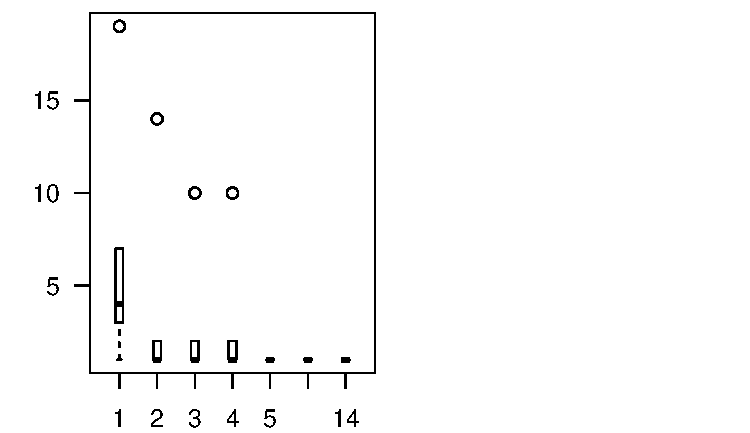
\includegraphics[scale=0.35,trim=10 0 130 0,clip]{R/idqaccess/idqaccess.pdf}
    \caption{idqaccess}
  \end{subfigure}%
  \begin{subfigure}{.2\textwidth}
    \centering
    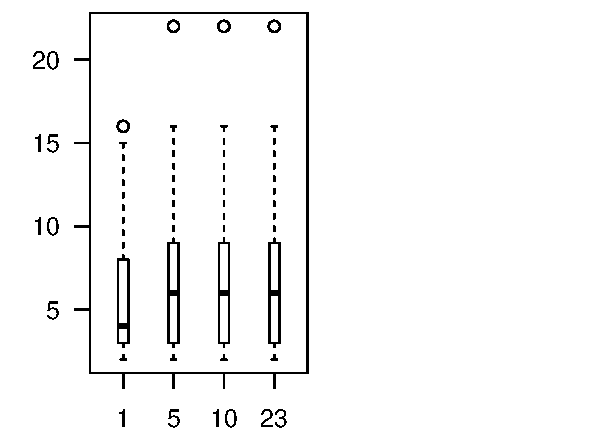
\includegraphics[scale=0.35,trim=15 0 130 0,clip]{R/scripttag/scripttag.pdf}       \caption{scripttag}    
  \end{subfigure}%
  \caption{\label{fig:impact-number-attacks}Impact of number of positive examples.}
  \vspace{-2ex}
\end{figure}

Figure~\ref{fig:impact-number-attacks} shows the results for each
attack we selected. The y-axis of each plot denotes the rank of the
golden rule and x-axis denotes the number of attack examples used to
synthesize rules. Each point in the x-axis is associated with the
boxplot of the distribution for the corresponding number of
variants. Results indicate that the number of examples is important,
the choice of examples is important, and a small number of examples
suffices to reach the best results.

\begin{figure}[h!]
  \vspace{-1.5ex}
  \centering
  \begin{subfigure}{.2\textwidth}
    \centering
    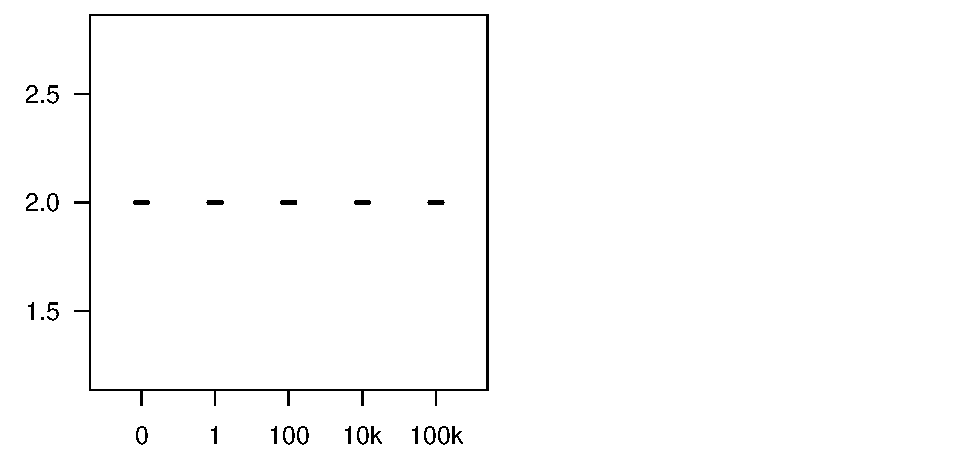
\includegraphics[scale=0.35,trim=10 0 130 0,clip]{R/coldfusion/coldfusion.pdf}
    \caption{coldfusion}
  \end{subfigure}%
  \hspace{-8ex}
  \begin{subfigure}{.2\textwidth}
    \centering
    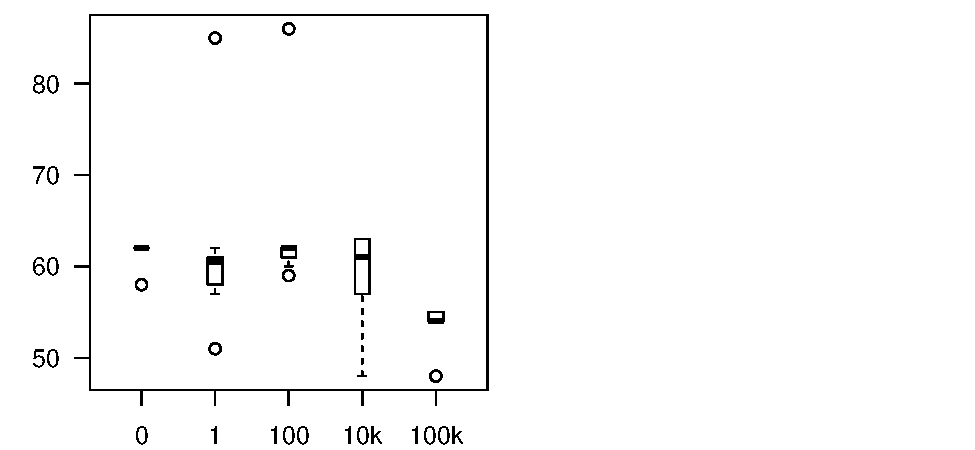
\includegraphics[scale=0.35,trim=15 0 130 0,clip]{R/inc/inc.pdf}
    \caption{inc}    
  \end{subfigure}%
  \hspace{-8ex}
  \begin{subfigure}{.2\textwidth}
    \centering
    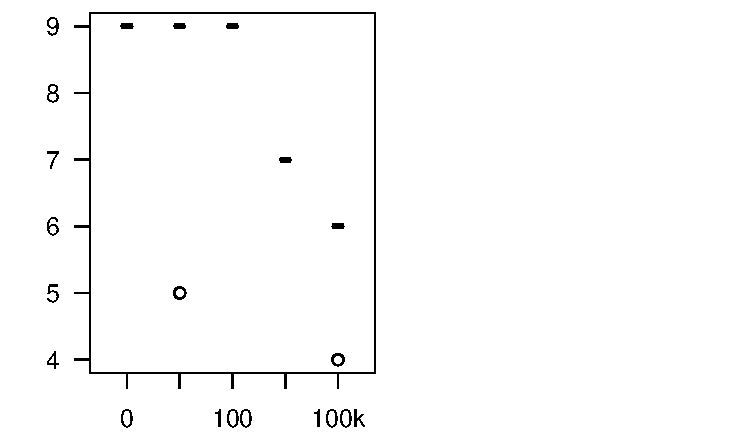
\includegraphics[scale=0.35,trim=15 0 130 0,clip]{R/jsp/jsp.pdf}
    \caption{jsp}    
  \end{subfigure}%
  \caption{Impact of number of negative examples.}
  \label{fig:impact-negative}
  \vspace{-2ex}
\end{figure}

We conducted a similar experiment with negative examples on three
different attacks. Figure~\ref{fig:impact-negative} shows
results. Note that, compared with the plots of
Figure~\ref{fig:impact-number-attacks}, the rank of the golden rule
improves at a much slower pace. Fortunately, negative traffic is much
easier to access.

%% \begin{center}
%% \begin{tcolorbox}[enhanced,width=3.5in,center upper,drop shadow southwest,sharp corners]

%% \end{tcolorbox}
%% \end{center}

\emph{ \textbf{Summary of results:}~\tname\ is sensitive to the number
  and choice of examples. However, a small number of positive examples
  suffices to achieve good results.}

%% \pgfplotsset{
%%   box plot width/.initial=0.5em
%% }
%% \begin{tikzpicture}
%%   \begin{axis}
%%     [
%%     ytick={1,2,3},
%%     yticklabels={Index 0, Index 1, Index 2},
%%     ]
%%     \addplot+[
%%     boxplot prepared={
%%       median=1,
%%       upper quartile=1.2,
%%       lower quartile=0.4,
%%       upper whisker=1.5,
%%       lower whisker=0.2
%%     },
%%     ] coordinates {};
%%     \addplot+[
%%     boxplot prepared={
%%       median=2,
%%       upper quartile=2.3,
%%       lower quartile=1.5,
%%       upper whisker=2.7,
%%       lower whisker=1
%%     },
%%     ] coordinates {};
%%     \addplot+[
%%     boxplot prepared={
%%       median=0.7,
%%       upper quartile=1.4,
%%       lower quartile=0.5,
%%       upper whisker=1.9,
%%       lower whisker=0.1
%%     },
%%     ] coordinates {};
%%   \end{axis}
%% \end{tikzpicture}

%\subsection{Threats to Validity}

\subsection{Discussion}
\label{sec:rce}
\label{sec:jboss}
\label{sec:content-example}
\label{sec:dos}
\label{sec:threats}

%\subsubsection{Lack of comparison with other tools}
\noindent\textbf{Lack of comparison with other tools}
Table~\ref{table:comparison} summarizes the characteristics of
alternative techniques and provides details about the evaluation used
in corresponding papers. Unfortunately, side comparison was not
possible for three key reasons. First, we did not have access to the
tools. We tried, unsuccssefully, making contact with authors to obtain
the tools. Second, the tools output different objects. For that
reason, a comparison based on published results did not make sense. It
is important to recall that we did not report precision and recall as
it is 100\% always. \tname captures, by construction, all positive
traffic and does not capture any negative traffic. We used a stronger
criteria instead---the position of the correct rule in the ranking. It
is possible that other rules, higher in the ranking, are useful, but
only domain experts can identify that. Third, we are the only
technique to support content options, which are prevalent and
challenging to handle. A side comparison would be unfair if we
consider rules with those options.
\noindent\textbf{Running times.}~We ran all our tests using an
Intel(R) Xeon(R) CPU E3-1240 v6 and 8GB RAM. For attacks with only
categorical and numerical options, the average running time was 6
seconds per attack. For attacks with the content option, the average
running time was 1,445 seconds (=24.1 minutes).  \textbf{Threats to
  Validity.}~Considering external validity. Our results cannot be
generalized beyond the subjects we selected. To mitigate that threat
we selected a variety of attacks with different
characteristics. Unfortunately, we could not access tools for related
techniques, but there is strong evidence that \tname\ performs very
well and is the only technique to support content options, which are
very important in this domain. Considering internal validity, in
principle, the implementation of \tname\ could contain errors. We
mitigated that threat by carefully inspecting code and
results. Considering construct validity, the choice of ranking to
evaluate the approach may not be useful in practice. We considered the
use of ranking of the golden rule a reasonable choice as the approach
places the golden rule close to the top in most cases.

% For that reason, we made a side-comparison based on the common
% examples and results reported in the original paper. 

%%  \Gui{There are a few reasons that makes the comparison between Syrius and other tools impossible 

%% \textbf{Tools availability.} We tried contact with authors of 4 different papers \cite{vollmer-etal-cics2011}\cite{muthuregunathan-etal2009}\cite{fallahi}\cite{Kao2015AutomaticNR}, but got no response from them. Since their tools are not available online or at least not publicly, we could not run them.

%% \textbf{Different output and specific rules.} We considered using the results they provides with results that Syrius provide, but concluded it wouldn't be possible as the results are essentially different. Commonly the  other results focus on showing the ratio of false negatives and false positives as a way to show the efficiency of the learning algorithm, but never comparing the generated rules to a Ground Truth, and most of times not showing individually the attacks used. Syrius' results, on the other hand, shows the generated rules that produce no false positives and negatives to the given packets, and always compares the results with a Ground Truth to verify its efficiency.

%% \textbf{'content' option support.} Another limitation is the support of 'content' option. Most papers do not support rule generation with the 'content' option, using only classic DDoS attacks in the rule generation, like ICMP and SYN flood, which only use numerical and categorical options. Some papers do support 'content', but don't explain well how they handle those rules with exclusive 'content'.}
%%  \Luc{Vollmer \cite{vollmer-etal-cics2011} and Guruprasad \cite{guruprasad} used 
%%  evolutionaries approaches to 
%% autonomously generate rules using the Snort IDS. They built 
%% their own ICMP datasets by using packet creation tools or by capturing network traffic. 
%% Guruprasad also used DARPA 1999 \cite{darpa1999} and ISCX 2012 \cite{iscx} datasets 
%% for non-ICMP attacks.
%% 
%% Vollmer created ten different packets to match ten existing rules, and then used 
%% these packets as input to the rule generation process. As a result, the produced 
%% rules achieved a 100\% detection rate and produced 3 false positives out of 33k packets.
%% 
%% Guruprasad manually created a set of rules by analyzing the network patterns and 
%% the datasets, this set of rules was used as the initial population of the algorithm. 
%% The produced rules achieved a detection rate up to 96\%, the false positive rate 
%% was not evaluated. 
%% 
%% On our experiments with Syrius, we used a total of \totalPackets packets that 
%% matches \totalAttacks different existing rules and it was able to generate rules that detected 
%% all the packets with no false positives.  
%%  }  



%%%%%%%%%%%%%%%%%%%%%%%%%%%%%%%%%%%%%%%%%%%%%%%%%%%%%%%%%%%
%% Add this in a journal submission in section to discuss
%% limitations...
%%%%%%%%%%%%%%%%%%%%%%%%%%%%%%%%%%%%%%%%%%%%%%%%%%%%%%%%%%%

%% \begin{figure}[t!]
%%   \lstinputlisting[language=C,numbers=none,keywords={content,flow}]{adaptor-golden-rule.suricata}
%%   \caption{\label{fig:rule-jboss}Suricata rule for JBoss Remote Code
%%     Execution.}
%% \end{figure}

%% \Mar{We may want to comment part of this to make room for the 
%%   experiments that Lucas and Guilherme are currently running.
%%   Side-comparison with prior work based on paper (not actual tool) results.}
%% This section elaborates how \tname\ performs on two other attacks.
%% \textbf{Remote Code Execution (RCE).}~RCE refers to the family of
%% attacks where hackers exploit a network vulnerability to run arbitrary
%% code on a remote machine. The code to be executed could damage the
%% system or steal sensitive information. JBoss~\cite{jboss} is a popular
%% open source Java application server. This attack enables remote
%% execution of code on the JBoss application server.
%% Figure~\ref{fig:rule-jboss} shows a Suricata rule that captures a
%% JBoss RCE attack.  The option \CodeIn{flow: established, to\_server;}
%% indicates that a rule match will only occur on packets that (1) flow
%% on an already-established connection and that (2) flow to the server
%% as opposed to the client. For the content options the modifiers
%% \CodeIn{nocase} and \CodeIn{http\_uri} indicate, respectively, that
%% the matching is not case sensitive and that the string should be
%% located at the packet field ``Request URI''. We reproduced the
%% malicious JBoss attack using the traffic from a Nikto
%% script~\cite{nikto}. Similar attacks are also available on the
%% Metasploit database~\cite{metasploit}. This is a case where
%% \tname\ performed poorly. Of the 228 plausible rules it generated for
%% this attack, the ground truth was located at position 45 in the ranked
%% list.


%% \textbf{Denial-of-Service.}~
%% The SYN Flood attack is a denial-of-service attack that exploits a
%% vulnerability in the tcp/ip handshake
%% to establish a tcp connection~\cite{cloudfare-synflood}. The handshake
%% works as follows in normal circumstances. First, a client sends a SYN
%% packet to the server, requesting a connection. Second, the server
%% responds with a SYN-ACK packet to the client. Third, the client
%% responds with an ACK message and the connection is established. Aware
%% of the protocol, an attacker sends multiple SYN packets to different
%% ports of a server, often using fake IP addresses. Then, after the
%% server responds with a SYN-ACK packet, the client keeps sending other
%% SYN packets to avoid the connection to time out. Without proper
%% protection, the server accepts these malicious requests and eventually
%% legitimate requests cannot be satisfied due to resource exhaustion.

%% %\vspace{-1ex}
%% \begin{figure}[h!]
%%   \lstinputlisting[language=C,numbers=none,keywords={flags,threshold}]{synflood.suricata}
%% %  \vspace{-2ex}
%%   \caption{\suri\ rule for SYN Flood attack.}
%%   \label{fig:synflood-example}
%% \end{figure}
%% %\vspace{-2ex}

%% Figure~\ref{fig:synflood-example} shows a Suricata rule that captures
%% this attack. This rule was obtained from the Emerging Threats Open
%% Ruleset~\cite{emerging-threats-open}. The relevant options in the
%% rule appear in bold---the option \CodeIn{flags: S,12}, identifies a
%% SYN packet in a tcp packet and the option \CodeIn{threshold: type
%%   both, track by\_dst, count 5000, seconds 5} indicates that a high
%% volume of such packets should be requested in a short period of
%% time. The other options are for documentation purposes. This is a case
%% where \tname\ works very well, reporting the golden rule at the top
%% of the ranking.


\section{Related Work}

\Mar{mention something on ethical hacking.. ethical-hacking}

This section elaborates on the most similar work.

\noindent
\textbf{Alternative methods for rule synthesis.} We discuss in the
following techniques similar in goal to ours. Unfortunately, we could
not access the tools implementing the techniques for side
comparison. Nevertheless, we found that there are important
differences between our work and related work. Vollmer
\etal{}~\cite{vollmer-etal-cics2011} propose the use of search to
derive rules for Snort, which are very similar to \suri's.  \Fix{Their
approach focuses on icmp attacks.} \Gui{The dataset used by them consists of manually produced ICMP packets using packet creation tools.}. It models every field of the icmp
packet in the chromosome of candidate solutions (\ie{}, a rule) of a
genetic search. The initial population is a set of candidate solutions
that randomly combine options, modelling the packet fields. They show
that they were able to generate rules without false negatives and only
3 false positives across 33K benign packets. The key differences
between our work and Vollmer~\etal{}'s are 1) the support of different
protocols and 2) the use of ranking to discriminate alternative
plausible rules. As for 1, our approach supports a variety of
protocols and options that refer to message payloads which
significantly increase the search space. The icmp rules they generate only
refer to message fields (see Section~\ref{sec:rules-and-packets}).
\MyComment{\Luc{eh possivel incluir contents em regras icmp tb. o q a secao 2.3 
diz q \textbf{geralmente} as regras nao-http possuem apenas field options}. }
As for 2, our solution additionally ranks plausible options, which
contain \emph{no} false positives or negatives with respect to the
benign and mallicious traffic considered.

\Gui{Guruprasad \etal{}\cite{guruprasad} also proposes an evolutionary framework, creating their own ICMP dataset as Vollmer, but also using DARPA 1999 \cite{darpa1999} and ISCX 2012 \cite{iscx} datasets for non-ICMP attacks. The produced rules reported a detection rate up to 96\%. Although Guruprasad supports more protocols than Vollmer, our approach still supports more options and protocols, making both key differences considered when comparing with Vollmer also relevant with Guruprasad.} 

Muthuregunathan \etal{}~\cite{muthuregunathan-etal2009} propose a clustering method to
create rules. They characterize candidate solutions as a set of field
values and use a clustering algorithm---hybrid k-means partitioned
around menoids---to isolate malicious from benign
traffic. Subsequently, they optimize the formed clusters using genetic
algorithms and hill-climbing search. Ou approach differs from theirs
in the method used, results, and support for content
options. Kao~\etal~\cite{Kao2015AutomaticNR} proposed ARGS, a system
to synthesize http rules that take malicious traffic as input. ARGS
looks for a common pattern across the different inputs to define
rules. It does not take existing rules as input or benign
traffic. Consequently, false positive can be produced and need to be
handled manually by users. Our approach, in contrast, does not
generate false positives w.r.t. the input traffic. 

\Gui{Fallahi \etal{}\cite{fallahi} proposes a flow-based solution for automated rule generation. Instead of analyzing the packets individually, their algorithm investigates and creates the rules for flows in the network. The algorithm was tested using the ISCX 2012 dataset and showed good results in terms of precision, but it is limited to the type of attack. As it won't analyse individual details of each packet, it wouldn't be able to identify and generate rules for attacks that require detailed options, such as the HTTP PESC, RCE and LFI.}

%% \Luc{\textbf{Autonomous Rule Creation for Intrusion Detection} -
%% Usam o Snort e geram regras apenas para pacotes ICMP. O pacote
%% maligno tb eh sabido previamente e, assim como nos, eles
%% identificam todas as opcoes q podem ser usadas para identificar
%% esse pacote. A tecnica proposta utiliza algoritmos geneticos onde a
%% populacao inicial eh formada por regras q combinam aleatoriamente
%% todas essas opcoes. Eles foram capazes de gerar regras q n geram
%% falsos negativos e apenas 3 positivos entre 33k pacotes.}

%% \Gui{\textbf{Efficient Snort Rule Generation using Evolutionary computing for Network Intrusion Detection -} O metodo proposto por Raghavan eh baseado em Clustering utilizando algoritmos geneticos e Hill climbing para otimizar os clusters formados. Outros papers, citados no related works, tambem propuseram uma ideia semelhante, no [1][4][6] do paper de Raghban.
%% A arquitetura proposta pega traffic files em intervalos de tempo constante e clusteriza os pacotes utilizando algoritmo hibrido de k means e partitioning around medoids. Com clusters formados, ele otimiza usando algoritmos geneticos e hill climbing.
%% Eh entao criada uma regra que isola perfeitamente o cluster considerado como ataque. Quanto as opcoes, ele nao especifica quais, e nao deixa claro que considera content. O que ele fala eh que para lidar com dados continuos, como numero de bytes enviados numa conexao tcp, ele utiliza ranges com > e < ( maior que menor que). E para opcoes discretas sao consideradas todas e colocados como um OR.
%% Ou seja, a IA serve para separar o ataque do trafego normal, e a regra eh gerada "do nada" e aparentemente eh bem especifica.}

%% \Gui{\textbf{Automatic NIDS Rule Generating System for Detecting HTTP-like Malware Communication -} Apresenta um sintetizador de regras para trafego HTTP. O metodo eh bem parecido com o nosso no que se trata em utilizar trafego maligno separado para a criacao de regra, e utilizacao de trafego benigno para detectar falso positivo. O ponto eh que eles nao descrevem o metodo que utilizam para separar os contents. Alem disso, caso um falso positivo seja capturado, a regra deve ser manualmente ajustadas.
%% O paper possui algo interessante que o nosso nao possui. Ele eh
%% capaz de detectar clusters nas regras criadas e pre existentes,
%% sendo capaz de otimiza-las.}

\noindent
\textbf{Rule repair.}~Hallahan~\etal{}~\cite{8102263} propose to
repair firewall rules based on false positive detected by the
rules. Although firewall and \nids\ rules have differences and the
problem addressed is different---repair not synthesis---the work is
similar in spirit and inspiring. We remain to evaluate how \tname\ can
be used for repair. 

\Gui{Ganesan \etal{}\cite{ganesan} introduces an idea of generating new sets of rules based on modifications of existing rules. They used the community edition of snort rules from 2012 for the modifications and tested with the the pcap file from the MACCDC 2012 dataset. It was reported an increase in the number of alerts, but it wasn't analysed the false alarmrates for abduced rules. Their technique is parallel to the rule creation strategies, as the objective of the modified rules is to capture variations and evolutions of attacks.}

\noindent
\textbf{Anomaly-based intrusion detection.}
Cordy~\etal{}\cite{cordy-etal-issta19} propose the use of a genetic
algorithm to not only generate attack schemes capable of penetrating
the tested anomaly-based NIDS, but also repairing the NIDS to identify
the given attack scheme. Although our approach and theirs use machine
intelligence to detect attacks, anomaly-based and rule-based
\nids\ are complementary, as discussed on
Section~\ref{sec:background}.

%% \Gui{\textbf{Automated Repair By Example for Firewalls -} Ruzica repara e modifica regras de firewall a partir de uma entrada contendo exemplos ou behaviour. Embora firewalls e NIDS nao sejam exatamente a mesma coisa, a estrutura de regras contem muitas semelhancas, e a utilizacao de exemplos para modificar a regra pode ser comparado com nosso metodo de criacao de regras a partir de um pacote maligno (para ser sincero, nao vi muitas semelhancas com nosso paper, nao sei descrever mais)}

%% \Gui{\textbf{Search-based test and improvement of machine-learning-based anomaly detection systems -} o autor desenvolve uma ferramenta search-based que ira testar e explorar automaticamente vulnerabilidades em Anomaly-Based NIDS, e entao apresentando medidas preventivas contra o ataque recem criado atravez de attack schemes, que detectam apenas o ataque e com o minimo de falsos positivos possivel. Semelhante a nos, eles tambem utilizam trafego benigno para simular uma rede normal. (Os metodos preventivos sao para Anomaly-Based NIDS, nao sei como se encaixa no nosso paper tambem)}




\section{Conclusions}

Network Intrusion Detectors are an important defense mechanism against
networks attacks. This paper presents \tname{}, a novel approach to
generate rules for Rule-based \nids. \tname\ leverages positive and
negative traffic and examples of trusted rules to synthesize
rules. \tname{} is organized as a pipeline of three components that
1)~create an over-specified seed rule, 2)~derive plausible rules from
the seed, and 3)~rank plausible rules. Experimental results provide
early evidence showing that \tname\ is very promising. It was able to
rank the correct rule among the first five rules of the reported
ranking in \percTopFiveRanking\ of the cases we analyzed. The data set
containing our experimental artifacts is publicly accessible at
\ourdataset.

\rui{thinking out loud here: one of the motivations is that it is time-consuming
and troublesome to generate new rules. Time-consuming is not being addressed in 
the RQs and I think that, albeit it is difficult to conduct such a study, we 
shuold discuss it. I would think that mentinoing the human-on-the-loop (not in-the-loop)
should also be dscussed (this is more about the troublesomeness)}


\balance
%\bibliographystyle{ACM-Reference-Format}
\bibliographystyle{IEEEtran}
\bibliography{references}


\end{document}
